\documentclass[10pt,twocolumn,letterpaper]{article}

\usepackage{cvpr}
\usepackage{times}
\usepackage{epsfig}
\usepackage{graphicx}
\usepackage{amsmath}
\usepackage{amssymb}
\usepackage{subcaption}
\usepackage{multirow}
\usepackage{color}
\usepackage[space]{grffile}
\usepackage{array}
\newcolumntype{C}[1]{>{\centering\arraybackslash}p{#1}}
\usepackage{chngpage}


% Include other packages here, before hyperref.

% If you comment hyperref and then uncomment it, you should delete
% egpaper.aux before re-running latex.  (Or just hit 'q' on the first latex
% run, let it finish, and you should be clear).
\usepackage[pagebackref=true,breaklinks=true,letterpaper=true,colorlinks,bookmarks=false]{hyperref}
\usepackage[font=small,labelfont=bf,tableposition=top]{caption}

%\cvprfinalcopy % *** Uncomment this line for the final submission

\def\cvprPaperID{976} % *** Enter the CVPR Paper ID here
\def\httilde{\mbox{\tt\raisebox{-.5ex}{\symbol{126}}}}

% Pages are numbered in submission mode, and unnumbered in camera-ready
\ifcvprfinal\pagestyle{empty}\fi
\begin{document}
%\makeatletter 
%\let\@oldmaketitle\@maketitle% Store \@maketitle
%\renewcommand{\@maketitle}
%{
%{\@oldmaketitle% Update \@maketitle to insert... 
%\centerline{
%\begin{tabular}{c}
%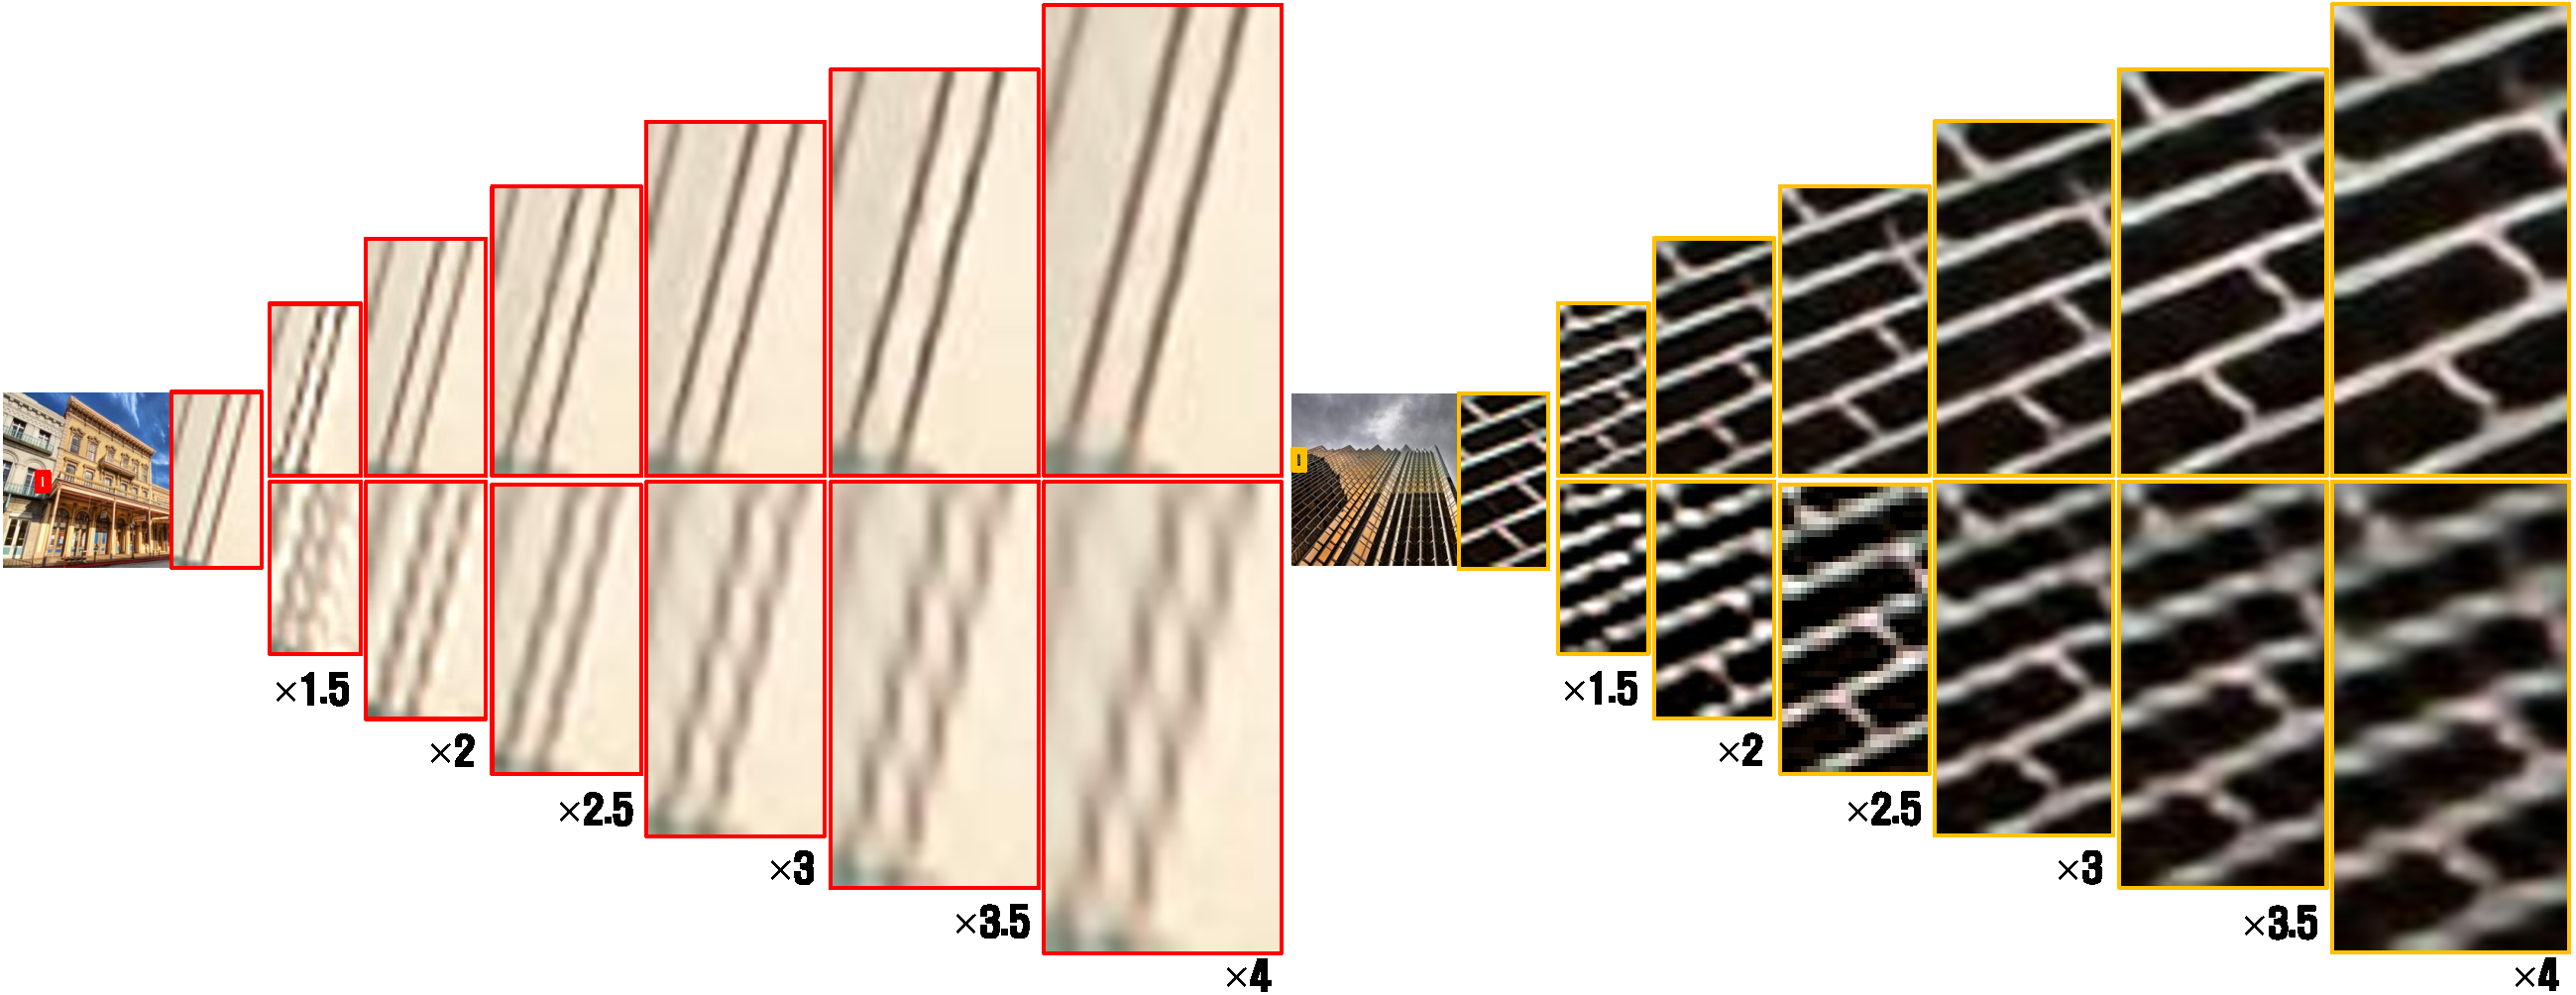
\includegraphics[width=\textwidth]{figs/fig1_sffsr.pdf}
%\end{tabular}
%%\begin{figure*}
%%\includegraphics{figs/sr10.png}
%%\end{figure*}
%}
%\bigskip}% ... an image 
%\vspace{-15pt}
%\captionof{figure}{\label{fig:fig1}
%(Top) Our results using a single network for all scale factors. Super-resolved images over all scales are clean and sharp. (Bottom)  Results of Dong et al.  \cite{Dong2014} ($\times$3 model used for all scales). Result images are not visually pleasing. To handle multiple scales, existing methods require multiple networks. }
%\vspace{15pt}
%}
%\makeatother


%%%%%%%%% TITLE
\title{Deeply-Recursive Convolutional Network for Image Super-Resolution}

\author{First Author\\
	Institution1\\
	Institution1 address\\
	{\tt\small firstauthor@i1.org}
	% For a paper whose authors are all at the same institution,
	% omit the following lines up until the closing ``}''.
	% Additional authors and addresses can be added with ``\and'',
	% just like the second author.
	% To save space, use either the email address or home page, not both
	\and
	Second Author\\
	Institution2\\
	First line of institution2 address\\
	{\tt\small secondauthor@i2.org}
}

\maketitle
%\thispagestyle{empty}

% TODO if net was trained very deep, it can be used in a shallow way for low-end PCs or mobiles


%%%%%%%%% ABSTRACT
\begin{abstract}
We propose an image super-resolution method (SR) using a deeply-recursive convolutional network (DRCN). Our network has a very deep recursive layer (up to 20 recursions). Increasing recursion depth can improve the performance without introducing new parameters for additional convolutions. Albeit advantages, learning a DRCN is very hard with a standard gradient descent method due to exploding/vanishing gradients. To ease the difficulty of training, we propose two extensions: recursive-supervision and skip-connection. Our method outperforms previous methods by a large margin.
\end{abstract}

%%%%%%%%% Figures Start
% Figures for the section 'Propose Method'
\begin{figure*}[t]
	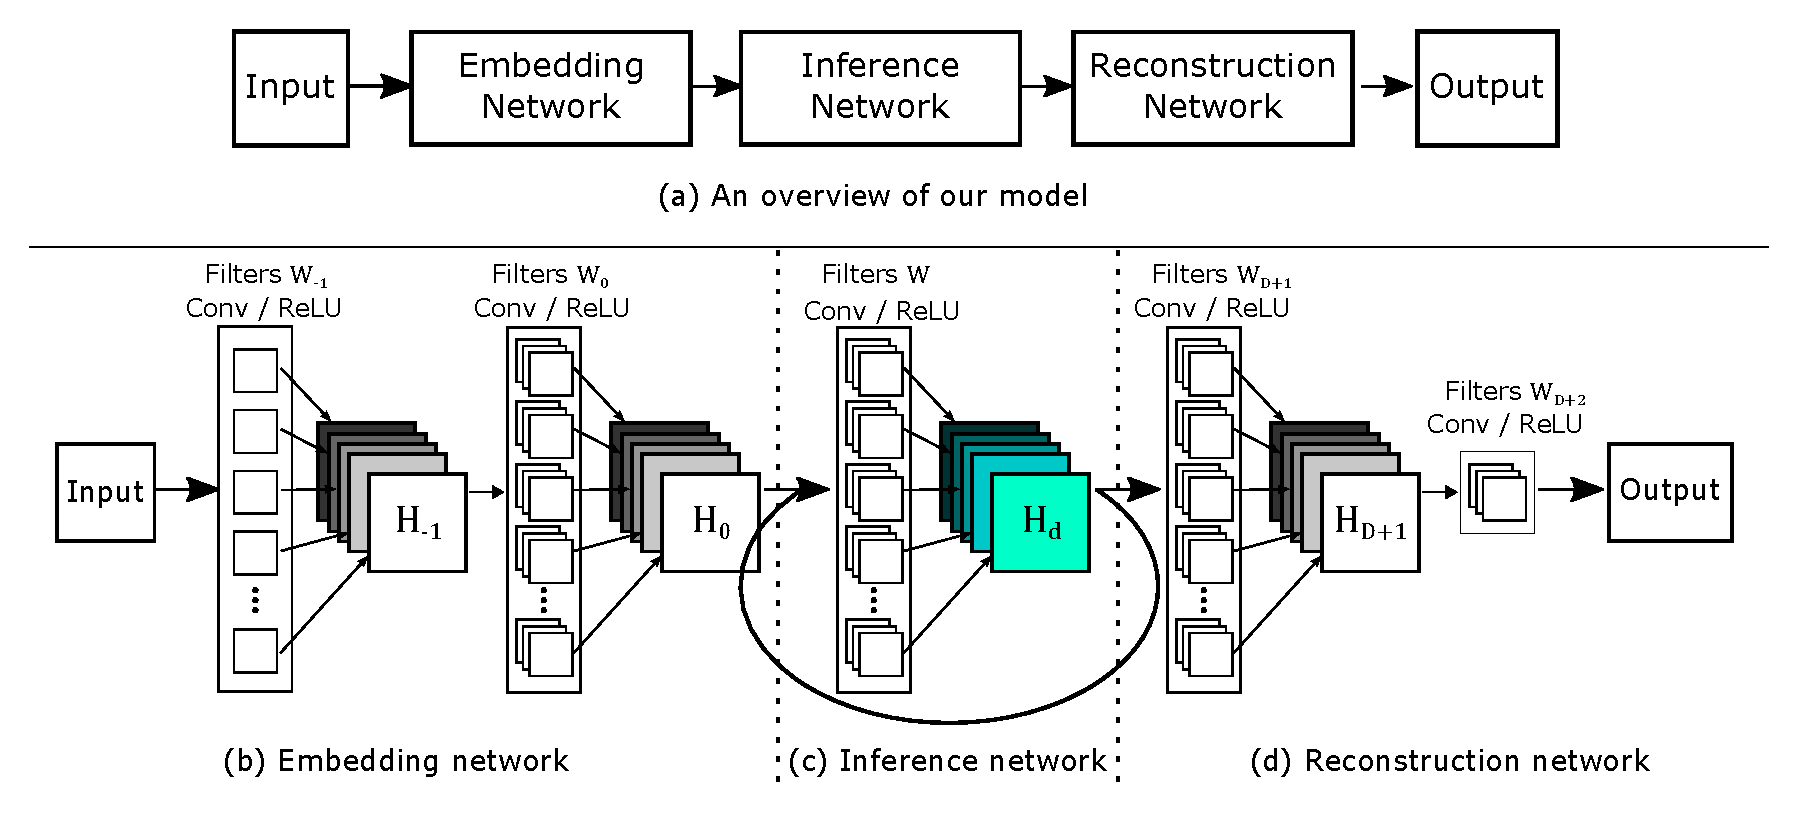
\includegraphics[width=\textwidth]{figs/f1}
	\caption {Architecture of our basic model. It consists of three parts: embedding network, inference network and reconstruction network. Inference network has a recursive layer and its unfolded version is in Figure \ref{fig:inference_network}.}
	\label{fig:overview}
\end{figure*}
%%%%%%%%% Figures End


%%%%%%%%% BODY TEXT
\section{Introduction}
For image super-resolution (SR), receptive field of a convolutional network determines the amount of contextual information that can be exploited to infer missing high-frequency components. For example, if there exists a pattern with smoothed edges contained in a receptive field, it is plausible the pattern is recognized and edges are appropriately sharpened. As SR is an ill-posed inverse problem, collecting and analyzing more neighbor pixels can possibly give more clues on what have been lost by downsampling. 

Deep convolutional networks (DCN) succeeding in various computer vision tasks often use very large receptive fields  (224x224 common in ImageNet classification \cite{krizhevsky2012imagenet, simonyan2015very}). Among many approaches to widen receptive field, increasing network depth is one possible way: A convolutional (conv.) layer  with filter size larger than $1\times 1$ or a pooling (pool.) layer that reduces the dimension of intermediate representation can be used.  Both approaches have drawbacks: a conv. layer introduces more parameters and a pool. layer typically discards some pixel-wise information. 

For image restoration problems such as super-resolution and denoising, image details are very important. Therefore, most deep-learning approaches for such problems do not use pooling. Increasing depth by adding a new weight layer basically introduces more parameters. Two problems can arise. First, overfitting is highly likely. More data are now required. Second, model becomes too huge to be stored and retrieved.


%[TODO Mention deep-learning SR methods.] A famous deep-learning SR method SRCNN \cite{Dong2014}, however, use only three layers resulting in a receptive field of 13 by 13. To utilize contextual information spread over very large image regions, many conv. layers need to be stacked in standard CNN settings. If $3 \times 3$ filters are stacked, stacking 10 layers result in $21 \times 21$ receptive field. This is still very small compared to typical image sizes.


To resolve the issues, we use a deeply-recursive convolutional network (DRCN). DRCN repeatedly applies the same convolutional layer as many times as desired. The number of parameters do not increase while more recursions are performed. Our network has the receptive field of 41 by 41 and this is relatively large compared to SRCNN \cite{dong2014image} (13 by 13). While DRCN has good properties, we find that DRCN optimized with the widely-used stochastic gradient descent method does not easily converge. This is due to exploding/vanishing gradients \cite{bengio1994learning}. Learning long-range dependencies between pixels with a single weight layer is very difficult. 

We propose two approaches to ease the difficulty of training (Figure \ref{fig:recursive_supervision}(a)). First, all recursions are simultaneously supervised. Feature maps after each recursion are used to reconstruct the target high-resolution image (HR). Reconstruction method (layers dedicated to reconstruction) is the same for all recursions. As each recursion leads to a different HR prediction, we combine all predictions resulting from different levels of recursions to deliver more accurate final prediction. The second proposal is to use a skip-connection from input to the reconstruction layer. In SR, low-resolution image (input) and high-resolution image (output) share the same information to a large extent. Exact copy of input, however, is likely to be attenuated during many forward passes. We explicitly connect the input to the layers for output reconstruction. This is particularly effective when input and output are highly correlated.

\textbf{Contributions} In summary, we propose an image super-resolution method deeply recursive in nature. It utilizes very large context compared to previous SR methods with only a single recursive layer. We improve the simple recursive network in two ways: recursive-supervision and skip-connection. Our method demonstrates the state-of-the-art performance in common benchmarks.

\section{Related Work}

\subsection{Single-Image Super-Resolution}

We apply DRCN to single-image super-resolution (SR) \cite{Irani1991, freeman2000learning,glasner2009super}. Many SR methods have been proposed in the computer vision community. Early methods use very fast interpolations but they give poor results. Some of more powerful methods utilize statistical image priors \cite{sun2008image,Kim2010} or internal patch recurrence \cite{glasner2009super, Huang-CVPR-2015}. Recently, sophisticated learning methods are widely used to model a mapping from LR to HR patches. Many methods have paid attention to find better regression functions from LR to HR images. This is achieved with various techniques: neighbor embedding \cite{chang2004super,bevilacqua2012}, sparse coding \cite{yang2010image,zeyde2012single,Timofte2013,Timofte}, convolutional neural network (CNN) \cite{dong2014image} and random forest \cite{schulter2015fast}.

Among several recent learning-based successes,  convolutional neural network (SRCNN) \cite{dong2014image} demonstrated the feasibility of an end-to-end approach to SR. One possibility to improve SRCNN is to simply stack more weight layers as many times as possible. However, this significantly increases more parameters and requires more data to prevent overfitting. In this work, we seek to design a convolutional network that models long-range pixel dependencies with limited capacity. Our network recursively widens receptive field without increasing the model capacity. 

\subsection{Recursive Neural Network in Computer Vision}

Recursive neural networks, suitable for temporal and sequential data, have seen limited use on algorithms operating on a single static image.   Socher et al.  \cite{socher2012convolutional} used a convolutional network in a separate stage to first learn features on RGB-Depth data, prior to hierarchical merging. In these models the input dimension is twice that of the output and recursive convolutions are applied only two times. Similar dimension reduction happens in the recurrent convolutional neural networks used for semantic segmentation \cite{pinheiro2014recurrent}. As SR methods predict full-sized images, dimension reduction is not allowed.

In Eigen et al. \cite{Eigen2014}, recursive layers have the same input and output dimension, but recursive convolutions resulted in worse performances than a single convolution due to overfitting. To overcome overfitting, Liang and Hu \cite{Liang_2015_CVPR} uses a recurrent layer that takes feed-forward inputs into all unfolded layers. They show that performance increases up to three convolutions. Their network structure, designed for object recognition, is the same as the existing CNN architectures.

Our network is similar to the above in the sense that recursive or recurrent layers are used with convolutions. We further increase the recursion depth and demonstrate that very deep recursions can significantly boost the performance for super-resolution. We apply the same convolution up to 16 times (previous maximum is three). 

%%%%%%%%% Figures Start
\begin{figure}[t]
	\includegraphics[width=0.5\textwidth]{figs/f2}
	\caption {Unfolding inference network. \textbf{Left}: A recursive layer \textbf{Right}: Unfolded structure. The same filter W is applied to feature maps recursively. Our model can utilize very large context without adding new weight parameters. }
	\label{fig:inference_network}
\end{figure}
%%%%%%%%% Figures End


%%% Figure Start
% This figure is for subsection 'Advanced Model'
\begin{figure*}[t]
\begin{center}
	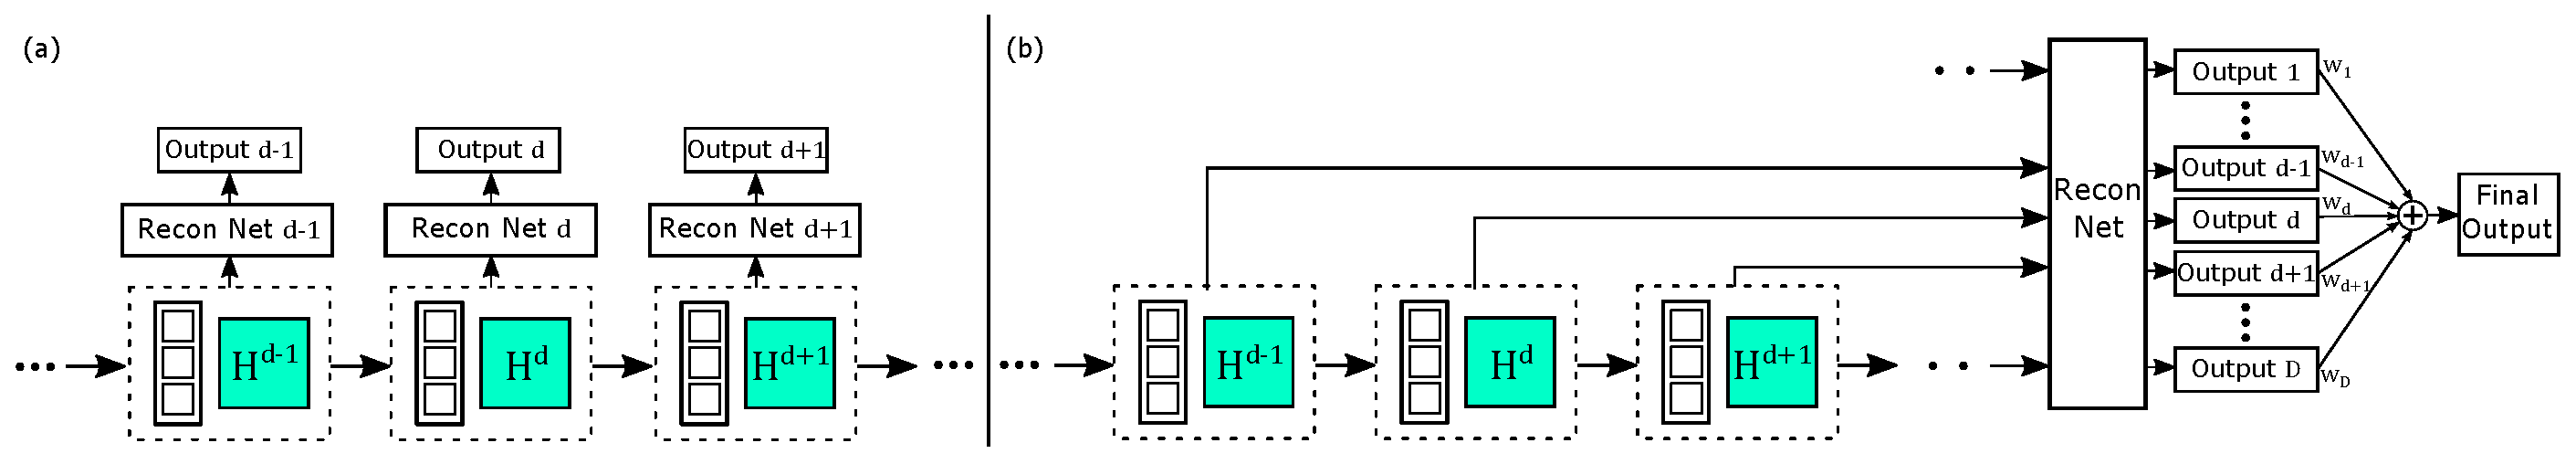
\includegraphics[width=\textwidth]{figs/f3}
	\caption{(a): Our final (advanced) model with recursive-supervision and skip-connection. The reconstruction network is shared for recursive predictions. We use all predictions from the intermediate recursion to get the final output. (b): Applying deep-supervision \cite{lee2014deeply} to our simple model. Unlike in (a), they use different reconstruction networks for recursions and more parameters are used.  (c) An example of expanded structure of (a) without parameter sharing (no recursion). The number of weight parameters is proportional to the depth squared. }
\label{fig:recursive_supervision}
\end{center}
\end{figure*}
%%% Figure End

\section{Proposed Method}
\subsection{Basic Model}

Our first model, outlined in Figure \ref{fig:overview}, consists of three sub-networks: embedding, inference and reconstruction networks. Embedding net is used to represent the given image as feature maps ready for inference. Next, inference net solves the task. Once inference is done, final feature maps in inference net are fed into reconstruction net to generate the output image.

\textbf{Embedding net} takes the input image (grayscale or RGB) and represent it as a set of feature maps. Intermediate representation used to pass information to inference net largely depends on how inference net internally represent its feature maps in their hidden layers. Learning this representation is done end-to-end altogether with learning other sub-networks. \textbf{Inference net} is the main component that solves the task, super-resolution. Analyzing a large image region is done by a single recursive layer. Each recursion applies the same convolution followed by a rectified linear unit (Figure \ref{fig:inference_network}). With convolution filters larger than $1\times 1$,  receptive field is widened every recursion. While feature maps from the final application of the recursive layer represent the high-resolution image, transformation of them (multi-channel) back into the original image space (1 or 3-channel) is necessary. This is done by \textbf{reconstruction net}.  

We have a single hidden layer for each sub-net. Only the layer for inference net is recursive. Other sub-nets are vastly similar to standard mutilayer perceptrons (MLP) with a single hidden layer. For MLP, full connection of $F$ neurons is equivalent to a convolution with $1\times 1\times F \times F$. In our sub-nets, we use $3\times 3\times F \times F$ filters. For embedding net, we use $3\times 3$ filters because image gradients are more informative than the raw intensities for super-resolution. For inference net, $3\times 3$ convolutions imply that hidden states are passed to adjacent pixels only. Reconstruction net also takes direct neighbors into account.

\textbf{Mathematical Formulation} The network takes an interpolated input image (to the desired size) as input ${\bf x}$ and predicts the target image ${\bf y}$ as in SRCNN \cite{dong2014image}. Our goal is to learn a model $f$ that predicts values $\mathbf{\hat{x}}=f(\mathbf{x})$. Let $f_1, f_2, f_3$ denote sub-net functions: embedding, inference and reconstruction, respectively. Our model is the composition of three functions: $f({\bf x}) = f_3(f_2 (f_1({\bf x}))).$
 
 Embedding net $f_1({\bf x})$ takes the input vector ${\bf x}$ and computes the matrix output $H_0$, which is an input to the inference net $f_2$. Hidden layer values are denoted by $H_{-1}$. The formula for embedding net is as follows:
  \begin{align}
        H_{-1} &= max(0, W_{-1}*{\bf x} + b_{-1})\\
        H_0 &= max(0, W_{0}*H_{-1} + b_0)\\
        f_1({\bf x}) &= H_0,
    \end{align}
where the operator $*$ denotes a convolution and $max(0,\cdot)$ corresponds to a ReLU. Weight and bias matrices are $W_{-1},W_0$ and $b_{-1},b_0$.

Inference net $f_2$ takes the input matrix $H_0$ and computes the matrix output $H_{D}$. Here, we use the same weight and bias matrices $W$ and $b$ for all operations.  Let $g$ denote the function modeled by a single recursion of the recursive layer: $g(H)=max(0,W*H+b)$. The recurrence relation is  
\begin{equation}
 H_d = g(H_{d-1}) = max(0,W*H_{d-1}+b),
\end{equation}
for $d = 1, ..., D$. 
Inference net $f_2$ is equivalent to the composition of the same elementary function $g$: 
\begin{equation}
f_2(H) = (g \circ g \circ \cdots \circ) g(H) =  g^{D}(H),
\end{equation}
where the operator $\circ$ denotes a function composition and $g^{d}$ denotes the $d$-fold product of $g$.

Reconstruction net $f_3$ takes the input hidden state $H_D$ and outputs the target image (high-resolution). Roughly speaking, reconstruction net is the inverse operation of embedding net. The formula is as follows:
\begin{align}
	H_{D+1} &= max(0, W_{D+1}*H_D + b_{D+1})\\
	\hat{{\bf y}} &= max(0, W_{D+2}*H_{D+1} + b_{D+2})\\
	f_3(H) &= \hat{{\bf y}}.
\end{align}

\textbf{Model Properties} Now we have all components for our model. The recursive model has pros and cons. While the recursive model is simple and powerful, we find training a deeply-recursive network very difficult. This is in accordance with the limited success of previous methods using at most three recursions so far \cite{Liang_2015_CVPR}.  Among many reasons, two severe problems are \textit{vanishing} and \textit{exploding gradients} \cite{bengio1994learning, pascanu2013difficulty}.  

\textit{Exploding gradients} refer to the large increase in the norm
of the gradient during training. Such events are due to
the multiplicative nature of chained gradients. Long term components can grow exponentially for deep recursions. The
\textit{vanishing gradients} problem refers to the opposite behavior. Long term components approach exponentially
fast to the zero vector. Due to it, learning a relation between distant pixels is very hard. Another known issue is that storing an exact copy of information through many recursions is very difficult. In training recurrent neural networks, relatively complex units such as LSTM TODO cite or GRU are used for long-term memory. In SR, output are vastly similar to input and recursive layer needs to keep the exact copy of input image for many recursions. These issues are also observed when we train our basic recursive model and we did not succeed in training a deeply-recursive network. 

In addition to gradient problems, there exists an issue with finding the optimal number of recursions. In theory, very large recursions are always good since the network sees more image region and we hope it learn to keep the important information and discard the unnecessary.  But in practice, a fixed-sized vector carrying all context information until the end of all recursions might lack capacity if recursions are too deep. To resolve the gradient and optimal recursion issues, we propose an improved model.

\subsection{Advanced Model} 
\textbf{Recursive-Supervision} We recursively-supervise all unfolded convolutions in order to alleviate the effect of vanishing/exploding gradients. As we have assumed that the same representation can be used again and again during convolutions in inference net, the same recon. net is used to predict HR images for all recursions. Our recon. net now outputs $D$ predictions and all predictions are simultaneously supervised during training (Figure \ref{fig:recursive_supervision} (a)). We use all $D$ intermediate predictions to compute the final output. All predictions are averaged during testing. The optimal weights are automatically learned during training. 

A similar but a different concept of supervising intermediate layers for a convolutional network is used in Lee et al  \cite{lee2014deeply}. Their method simultaneously minimizes classification error while improving the directness and transparency of the hidden layer learning process. There are two significant differences from our recursive-supervision to a deep-supervision proposed in Lee et al. \cite{lee2014deeply}. They associate an unique classifier for each hidden layer. For each additional layer, new classifier has to be introduced and new parameters thereby. If this approach is used, our modified network looks as in Figure \ref{fig:recursive_supervision}(b). Then we need $D$ different reconstruction networks. This is against our original purpose of using recursive networks: not introducing new parameters while stacking more layers. In addition, using different recon. nets no longer effectively regularizes the network. The second difference is that Lee et al. \cite{lee2014deeply} discard all intermediate classifiers during testing. However, an ensemble of all intermediate predictions significantly boosts the performance. The final output from the ensemble is also supervised.

Our recursive-supervision naturally eases the difficulty of training recursive networks. Backpropagation goes through a small number of layers if supervising signal goes directly from loss layer to early recursion. Summing all gradients backpropagated from different prediction losses give a smoothing effect. The adversarial effect of vanishing/exploding gradients along one backpropagation path is alleviated.

Moreover, the importance of picking the optimal number of recursions is reduced as our supervision enables utilizing predictions from all intermediate layers. If recursions are too deep for the given task, we expect the weight for late predictions low while early predictions receive high weights. By looking at weights of predictions, we can figure out the marginal gain from additional recursions. 

\textbf{Skip-Connection} Now we describe our second extension: skip-connection. For SR, input and output images are highly correlated. Carrying most if not all of input values until the end of the network is inevitable but very inefficient. Due to gradient problems, exactly learning a simple linear relation between input and output is very difficult if many recursions exists in between them.  

We add a layer skip \cite{bishop2006pattern} from input to the recon. net. Adding layer skips is successfully used for a semantic segmentation network \cite{long2014fully} and we employ a similar idea. Now input image is directly fed into the recon. net whenever it is used during recursions. Our skip-connection has two advantages. First, network capacity to store the input signal during recursions is saved. Second, the exact copy of input signal can be used during target prediction. 

Our skip-connection is simple yet very effective. In super-resolution, LR and HR images are vastly similar. In most regions, differences are zero and only small number of locations have non-zero values. For this reason, several super-resolution methods \cite{Timofte2013, Timofte, bevilacqua2012,bevilacqua2013super} predict image details only. Similarly, we find this domain-specific knowledge significantly improves our learning procedure. 

\textbf{Mathematical Formulation} Each intermediate prediction under recursive-supervision (Figure \ref{fig:recursive_supervision}) is 
\begin{equation}
\hat{{\bf y}}_{d} = f_3({\bf x}, g^{(d)}(f_1({\bf x}))),
\end{equation}
for $d=1,2,\dots,D$, where $f_3$ now takes two inputs, one from skip-connection. Recon. net with skip-connection can take various functional forms. For example, input can be concatenated to the feature maps $H_d$. As the input is an interpolated input image (roughly speaking, $\hat{\bf y} \approx {\bf x}$), we find $f_3({\bf x}, H_d) = {\bf x} + f_3(H_d)$ is enough for our purpose. More sophisticated functions for merging two inputs to $f_3$ will be explored in the future. 

Now, the final output is the weighted average of all intermediate predictions:
\begin{equation}
\hat{{\bf y}}^{(final)} = \sum_{d=1}^{D} w_d \cdot \hat{{\bf y}}_d.
\end{equation}
where $w_d$ denotes the weights of predictions reconstructed from each intermediate hidden state during recursion. These weights are learned during training.


%%%%%%%% Table Start
\begin{table*}
\begin{center}
\setlength{\tabcolsep}{2pt}
\footnotesize
\begin{tabular}{ | c | c | c | c | c | c | c | c | }
\hline
\multirow{2}{*}{Dataset} & \multirow{2}{*}{Scale} & Bicubic & A+ & SRCNN & RFL & SelfEx & DRCN (Ours)\\
 & & PSNR/SSIM & PSNR/SSIM & PSNR/SSIM & PSNR/SSIM & PSNR/SSIM & PSNR/SSIM\\
\hline
\hline
\multirow{3}{*}{Set5} & $\times$2 & 33.66/0.9299 & 36.54/{\color{blue}0.9544} & {\color{blue}36.66}/0.9542 & 36.54/0.9537 & 36.49/0.9537 & {\color{red}37.35}/{\color{red}0.9575}\\
 & $\times$3 & 30.39/0.8682 & 32.58/0.9088 & {\color{blue}32.75}/0.9090 & 32.43/0.9057 & 32.58/{\color{blue}0.9093} & {\color{red}33.76}/{\color{red}0.9223}\\
 & $\times$4 & 28.42/0.8104 & 30.28/0.8603 & {\color{blue}30.48}/{\color{blue}0.8628} & 30.14/0.8548 & 30.31/0.8619 & {\color{red}31.27}/{\color{red}0.8804}\\
\hline
\hline
\multirow{3}{*}{Set14} & $\times$2 & 30.24/0.8688 & 32.28/0.9056 & {\color{blue}32.42}/{\color{blue}0.9063} & 32.26/0.9040 & 32.22/0.9034 & {\color{red}32.89}/{\color{red}0.9098}\\
 & $\times$3 & 27.55/0.7742 & 29.13/0.8188 & {\color{blue}29.28}/{\color{blue}0.8209} & 29.05/0.8164 & 29.16/0.8196 & {\color{red}29.74}/{\color{red}0.8311}\\
 & $\times$4 & 26.00/0.7027 & 27.32/0.7491 & {\color{blue}27.49}/0.7503 & 27.24/0.7451 & 27.40/{\color{blue}0.7518} & {\color{red}27.88}/{\color{red}0.7629}\\
\hline
\hline
\multirow{3}{*}{B100} & $\times$2 & 29.56/0.8431 & 31.21/0.8863 & {\color{blue}31.36}/{\color{blue}0.8879} & 31.16/0.8840 & 31.18/0.8855 & {\color{red}31.74}/{\color{red}0.8916}\\
 & $\times$3 & 27.21/0.7385 & 28.29/0.7835 & {\color{blue}28.41}/{\color{blue}0.7863} & 28.22/0.7806 & 28.29/0.7840 & {\color{red}28.77}/{\color{red}0.7964}\\
 & $\times$4 & 25.96/0.6675 & 26.82/0.7087 & {\color{blue}26.90}/0.7101 & 26.75/0.7054 & 26.84/{\color{blue}0.7106} & {\color{red}27.16}/{\color{red}0.7193}\\
\hline
\hline
\multirow{3}{*}{Urban100} & $\times$2 & 26.88/0.8403 & 29.20/0.8938 & 29.50/0.8946 & 29.11/0.8904 & {\color{blue}29.54}/{\color{blue}0.8967} & {\color{red}30.42}/{\color{red}0.9087}\\
 & $\times$3 & 24.46/0.7349 & 26.03/0.7973 & 26.24/0.7989 & 25.86/0.7900 & {\color{blue}26.44}/{\color{blue}0.8088} & {\color{red}27.08}/{\color{red}0.8268}\\
 & $\times$4 & 23.14/0.6577 & 24.32/0.7183 & 24.52/0.7221 & 24.19/0.7096 & {\color{blue}24.79}/{\color{blue}0.7374} & {\color{red}24.97}/{\color{red}0.7431}\\
\hline
\end{tabular}
\caption{Benchmark results. Average PSNR/SSIMs for scale factor $\times$2, $\times$3 and $\times$4 on datasets Set5, Set14, B100 and Urban100. {\color{red}Red color} indicates the best performance and {\color{blue}blue color} refers the second best.}
\label{tbl:benchmark}
\end{center}
\end{table*}
%%%% Table end

%%%%% Figures Start
\begin{figure*}
\begin{adjustwidth}{0cm}{-0.5cm}
\begin{center}
\small
\setlength{\tabcolsep}{5pt}
\begin{tabular}{ c C{3.5cm}  C{3.5cm}  C{3.5cm}  }
\multirow{4}{*}{\graphicspath{{figs/fig1/}}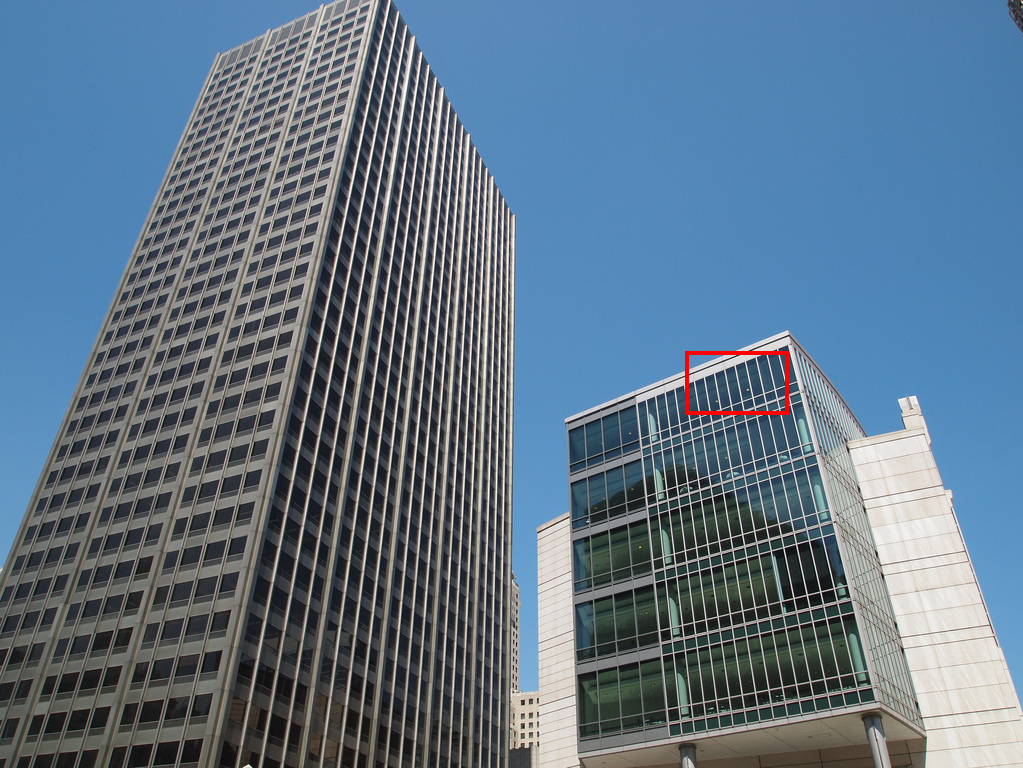
\includegraphics[width=0.27\textwidth]{img096_GTbox.png}}
& \raisebox{-13.0ex} {\graphicspath{{figs/fig1/}}
\includegraphics[width=0.20\textwidth]{img096_for_fig1_HR.png}}\vspace{0.3ex}
& \raisebox{-13.0ex} {\graphicspath{{figs/fig1/}}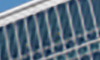
\includegraphics[width=0.20\textwidth]{img096_for_fig1_A+.png}}\vspace{0.3ex}
& \raisebox{-13.0ex} {\graphicspath{{figs/fig1/}}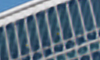
\includegraphics[width=0.20\textwidth]{img096_for_fig1_SRCNN.png}}\vspace{0.3ex}
\\
& Original (PSNR, SSIM)& A+ (23.99, 0.8320)& SRCNN (24.74, 0.8459)\\
& \raisebox{-13.0ex} {\graphicspath{{figs/fig1/}}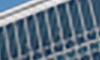
\includegraphics[width=0.20\textwidth]{img096_for_fig1_RFL.png}}\vspace{0.3ex}
& \raisebox{-13.0ex} {\graphicspath{{figs/fig1/}}
\includegraphics[width=0.20\textwidth]{img096_for_fig1_SelfEx.png}}\vspace{0.3ex}
& \raisebox{-13.0ex} {\graphicspath{{figs/fig1/}}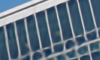
\includegraphics[width=0.20\textwidth]{img096_for_fig1_RCN.png}}\vspace{0.3ex}
\\
& RFL (23.95, 0.8230)& SelfEx (25.46, 0.8635)& DRCN (Ours) (26.25, 0.8933)\\
\end{tabular}
\caption{Super-resolution results of ``img096" (Urban100) with scale factor $\times$3. Patterned lines are straitened and sharpened in our result, whereas other methods give blurry lines. Our result seems visually pleasing.}
\label{fig:img1}
\end{center}
\end{adjustwidth}
\end{figure*}

\begin{figure*}
\begin{adjustwidth}{0.5cm}{0.5cm}
\begin{center}
\small
\setlength{\tabcolsep}{3pt}
\begin{tabular}{  c  c  c  c  c  c  }
{\graphicspath{{figs/fig2/}}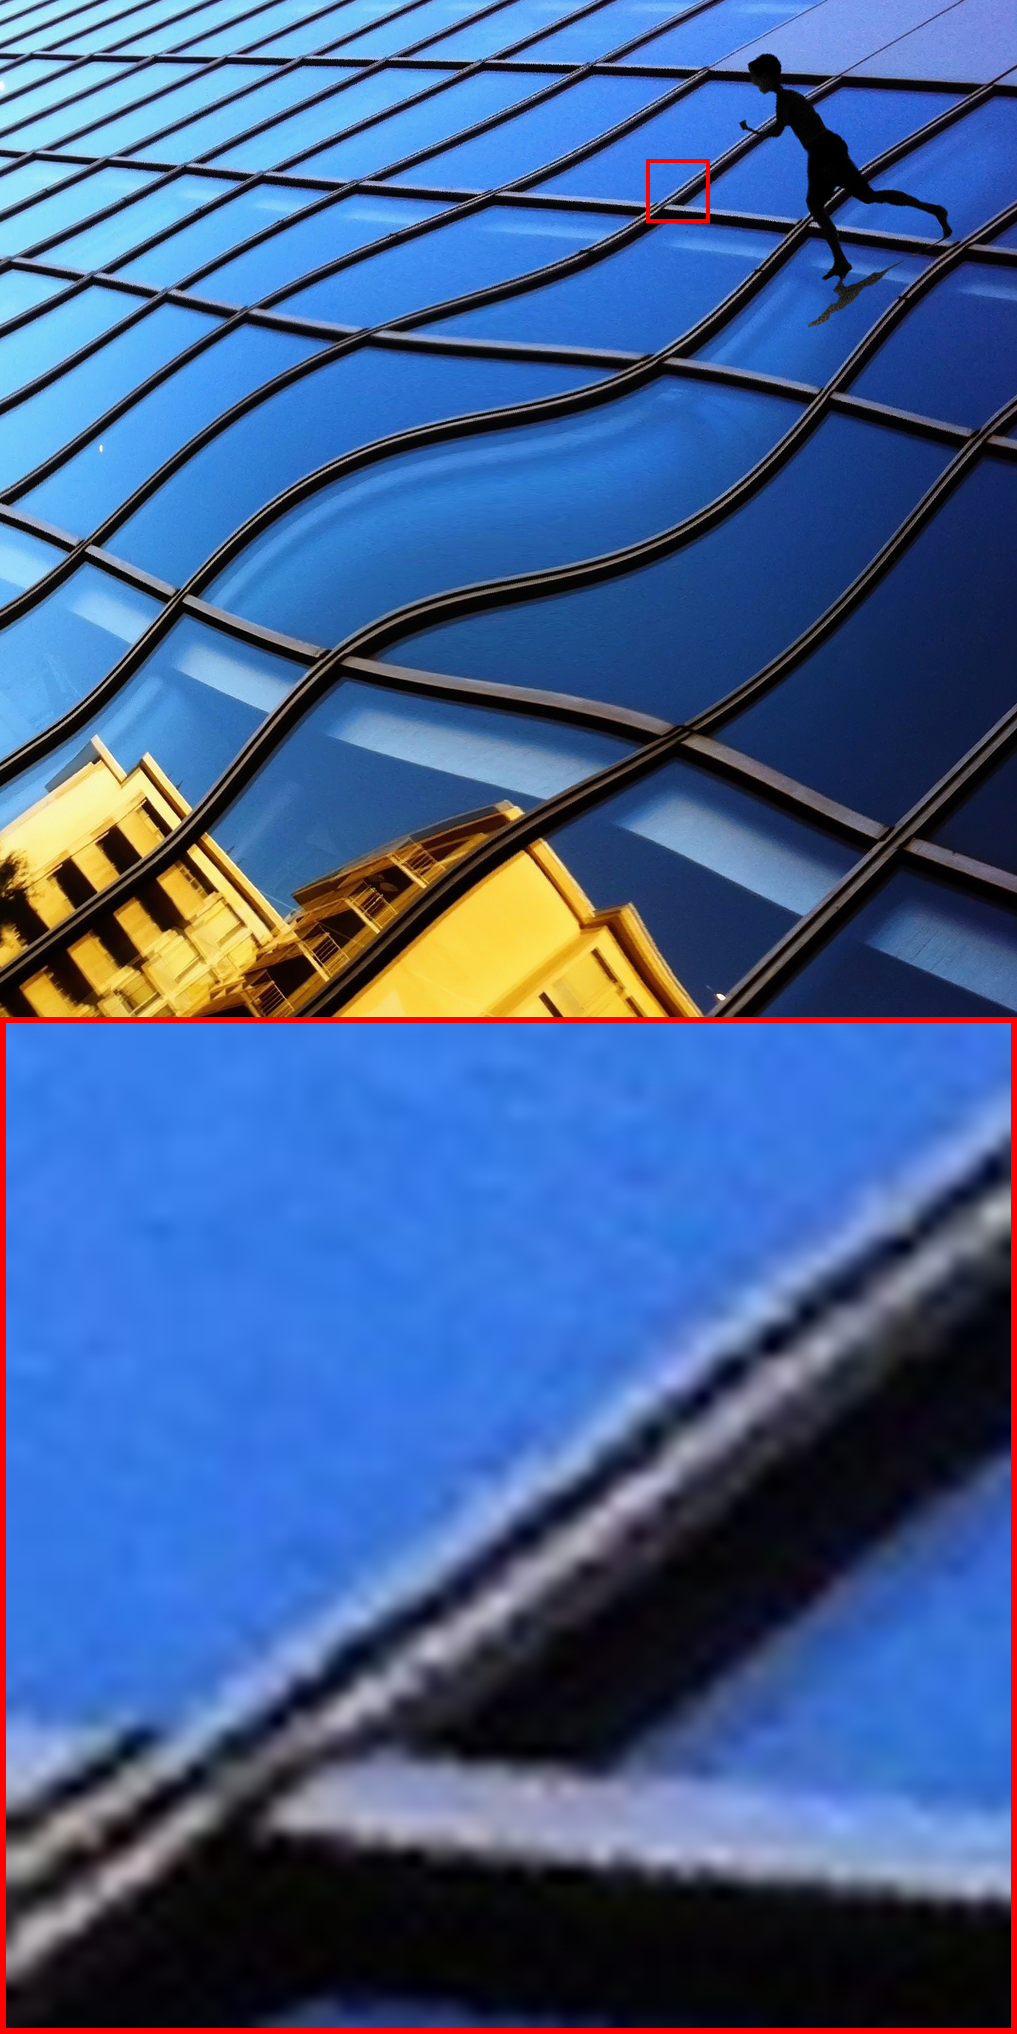
\includegraphics[width=0.15\textwidth]{img082_for_fig2_HR.png}}
& {\graphicspath{{figs/fig2/}}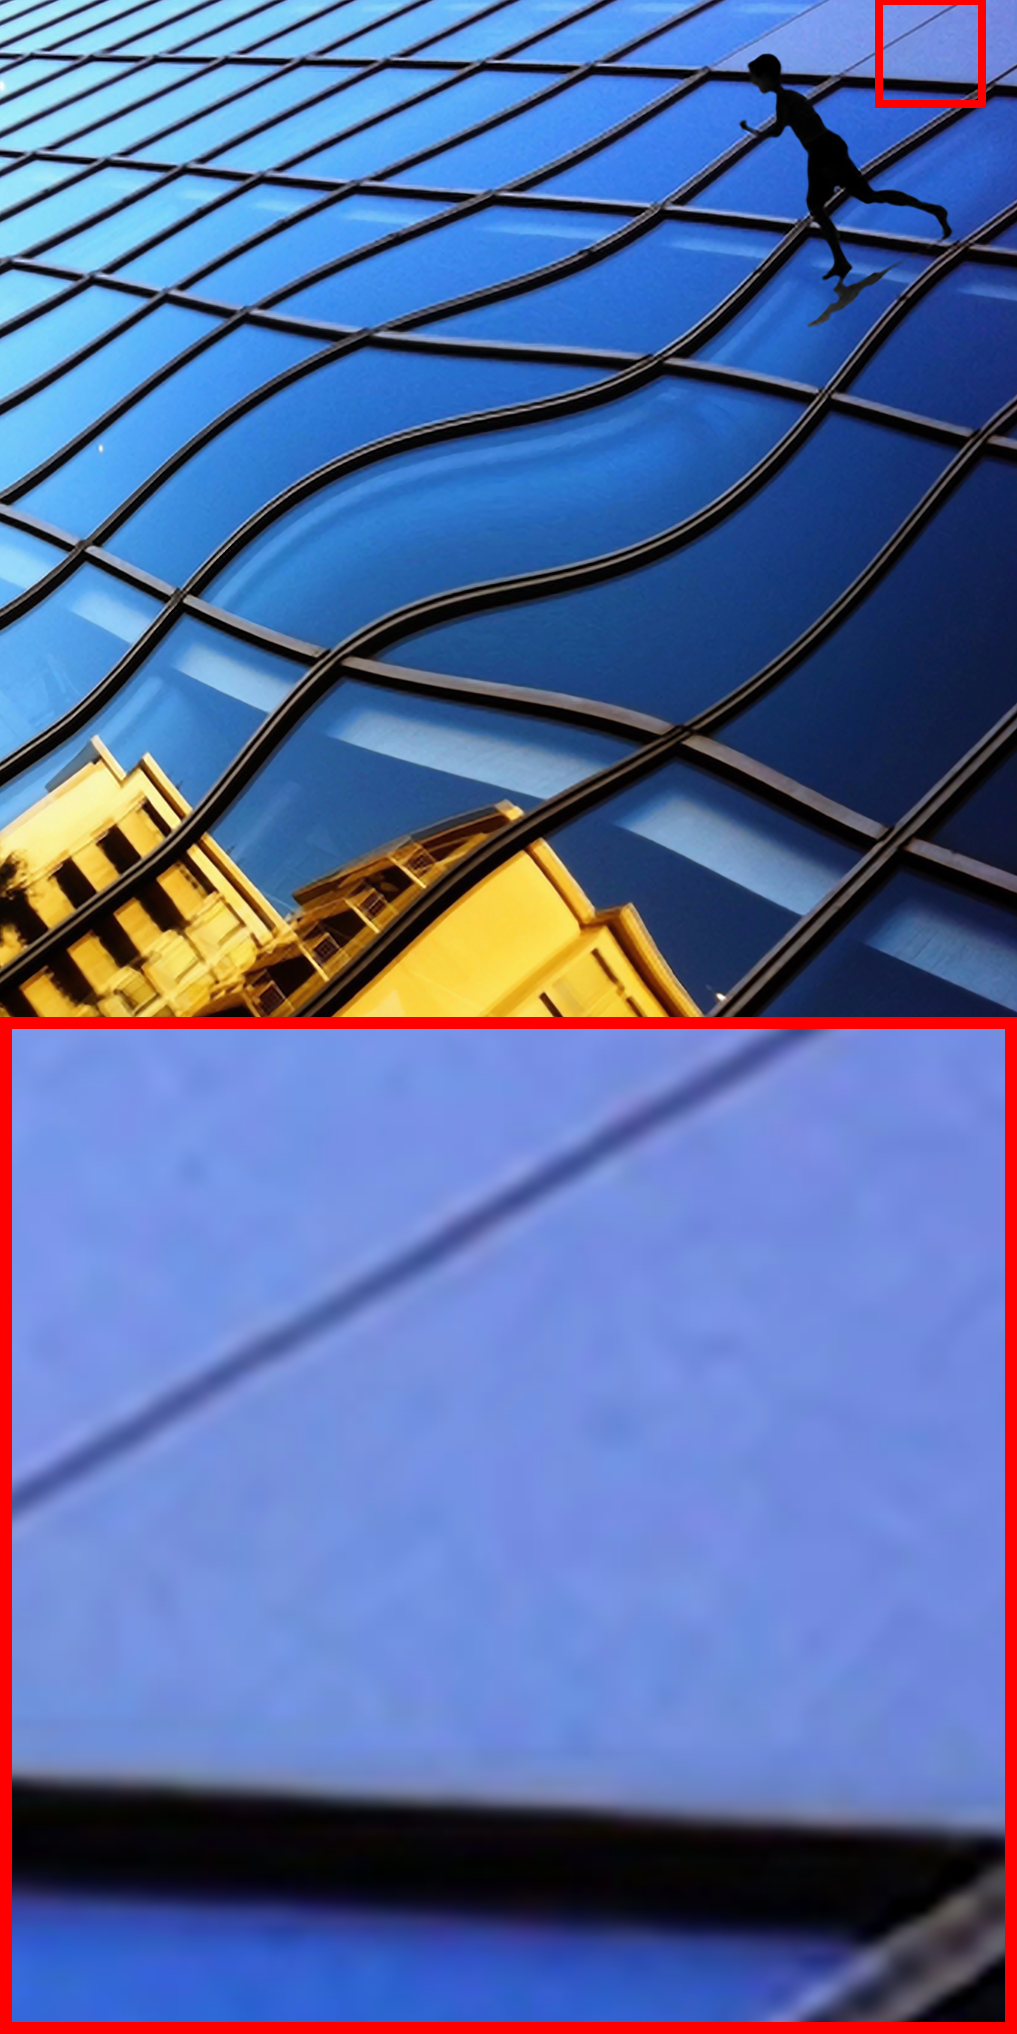
\includegraphics[width=0.15\textwidth]{img082_for_fig2_A+.png}}
& {\graphicspath{{figs/fig2/}}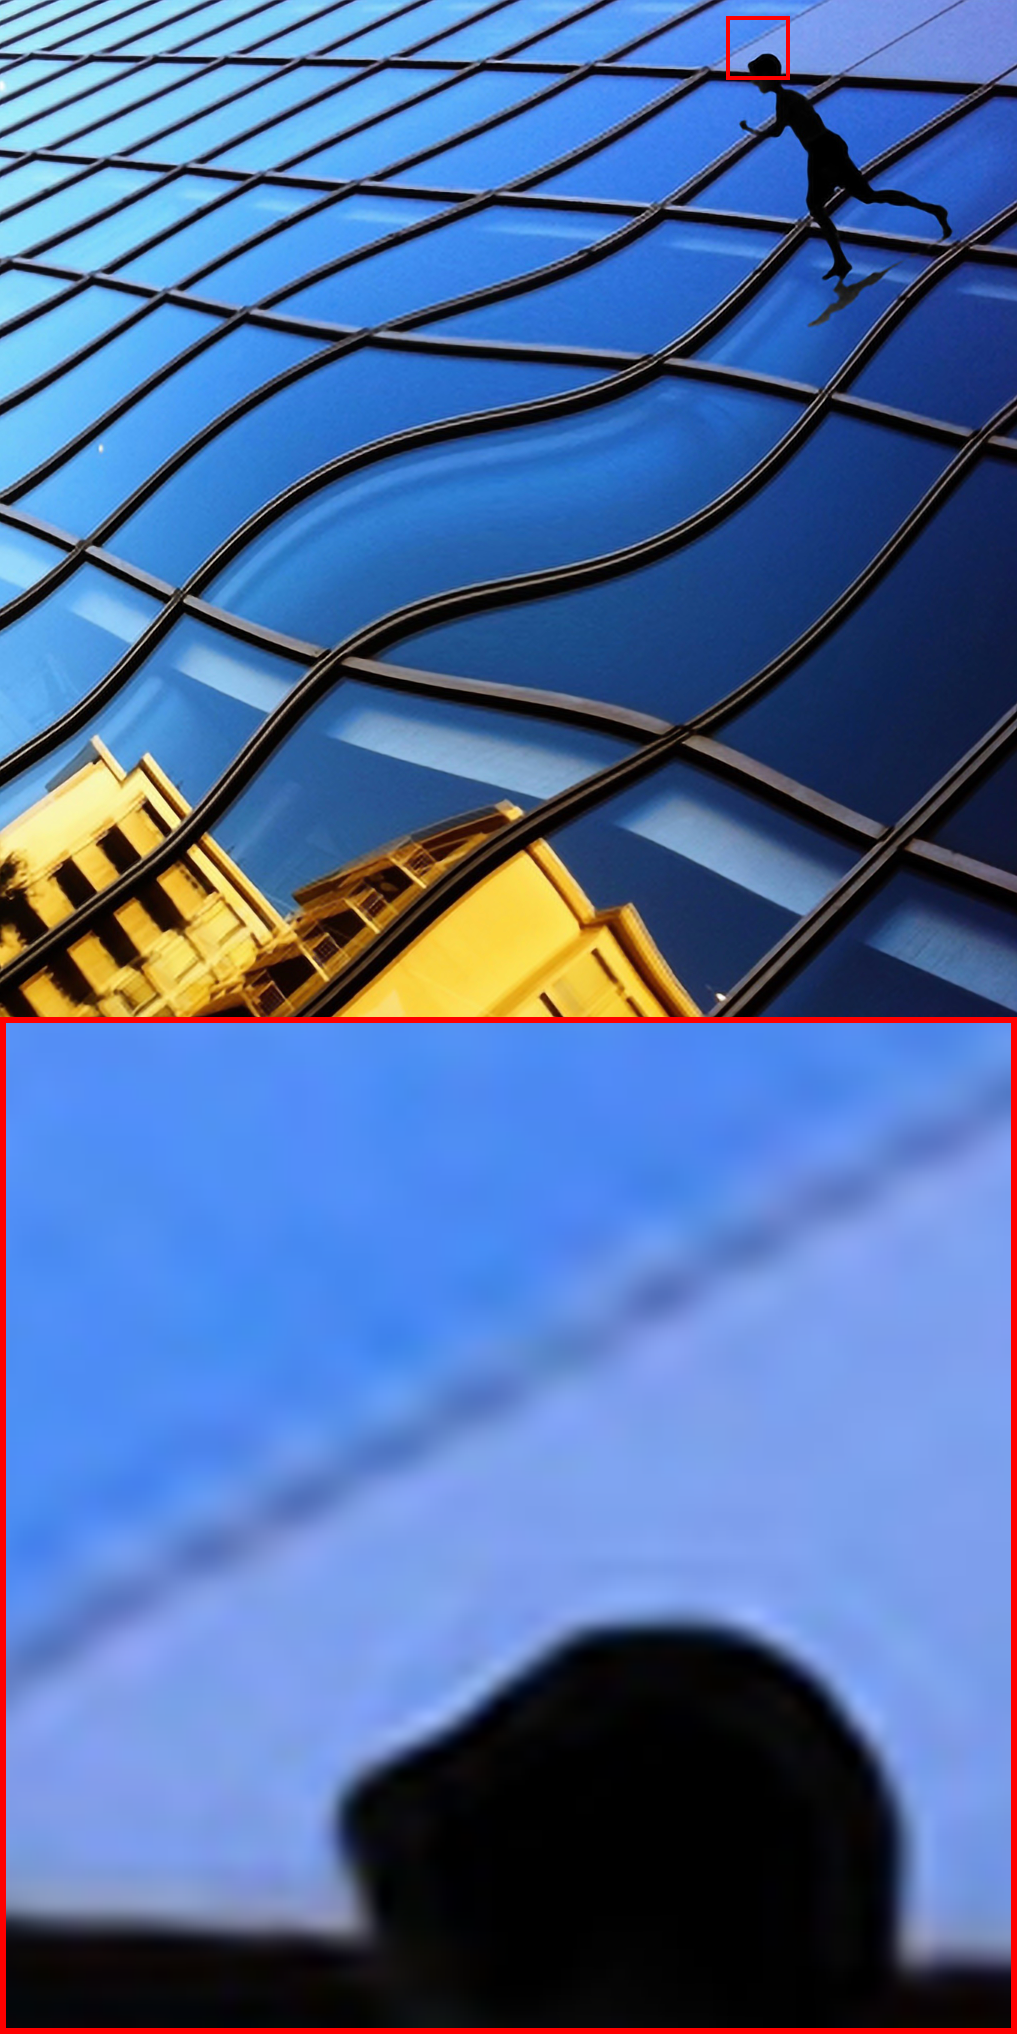
\includegraphics[width=0.15\textwidth]{img082_for_fig2_SRCNN.png}}
& {\graphicspath{{figs/fig2/}}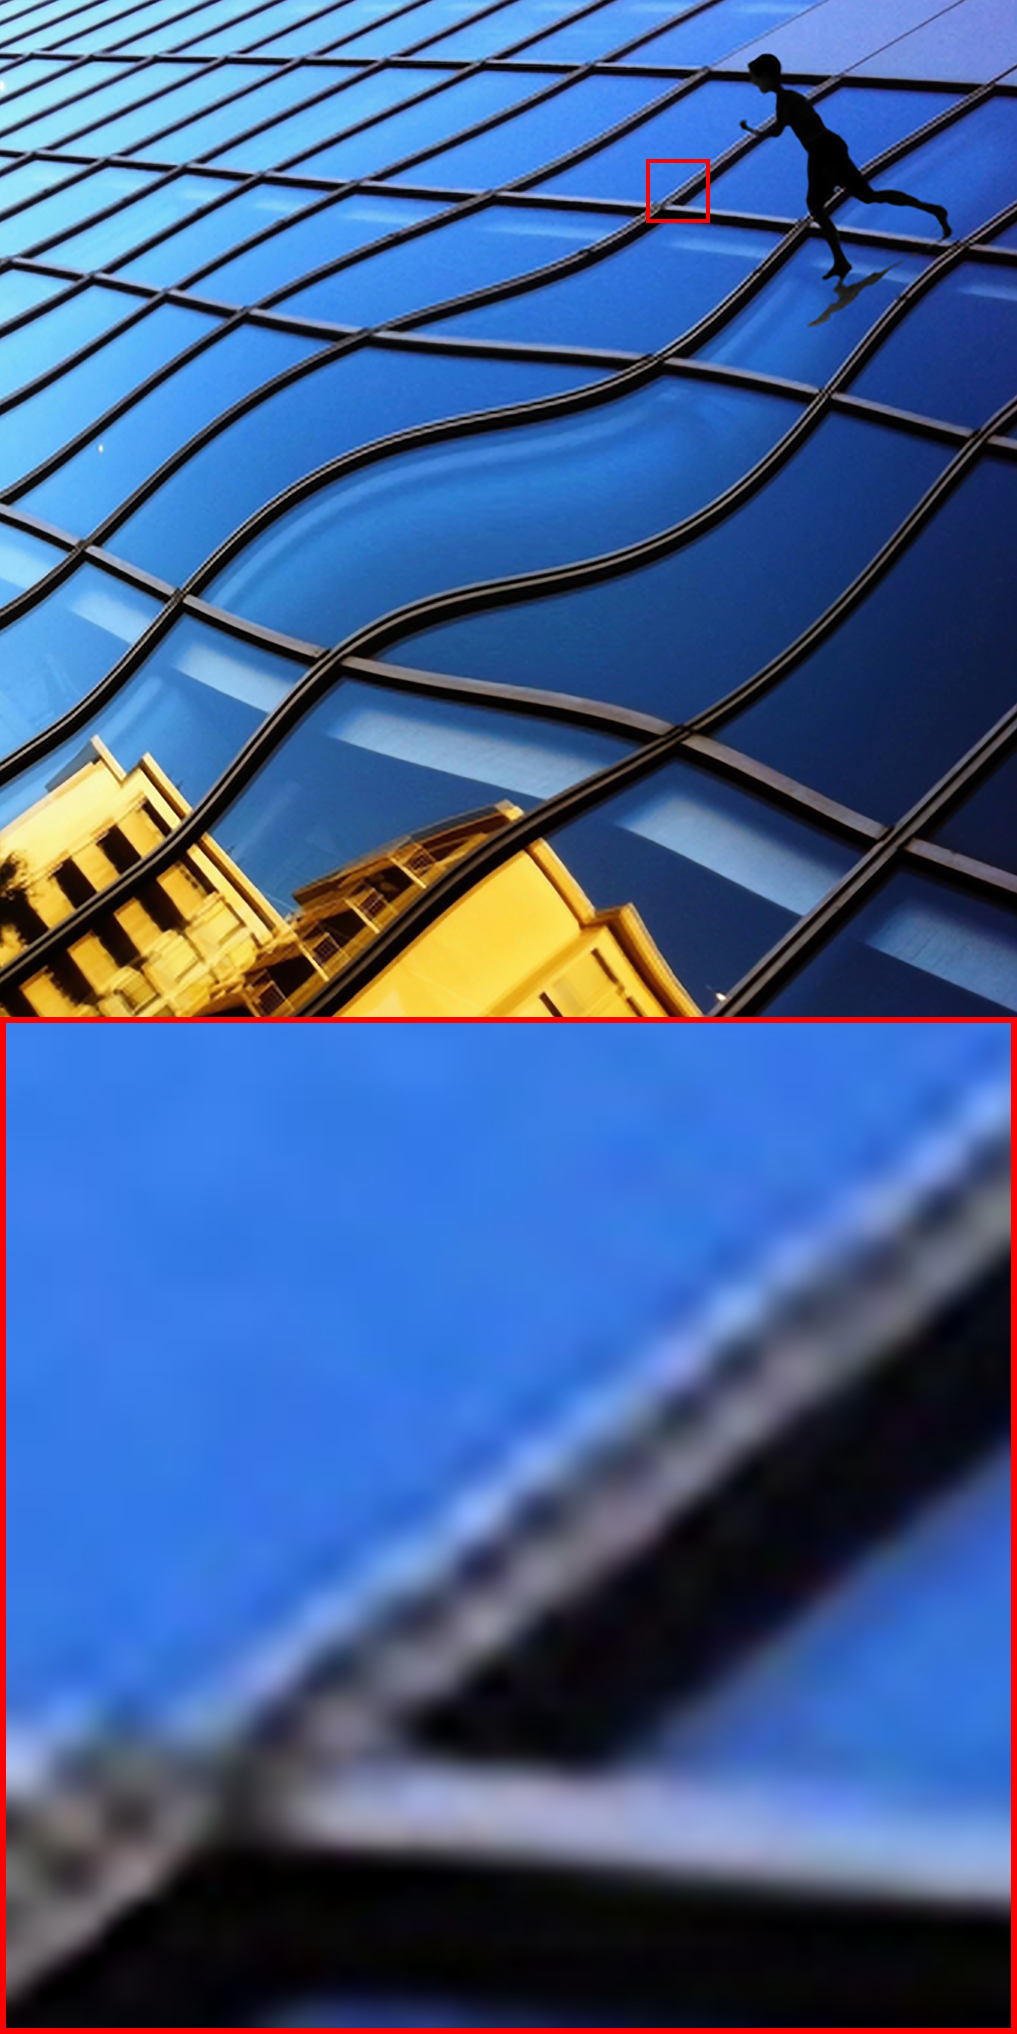
\includegraphics[width=0.15\textwidth]{img082_for_fig2_RFL.png}}
& {\graphicspath{{figs/fig2/}}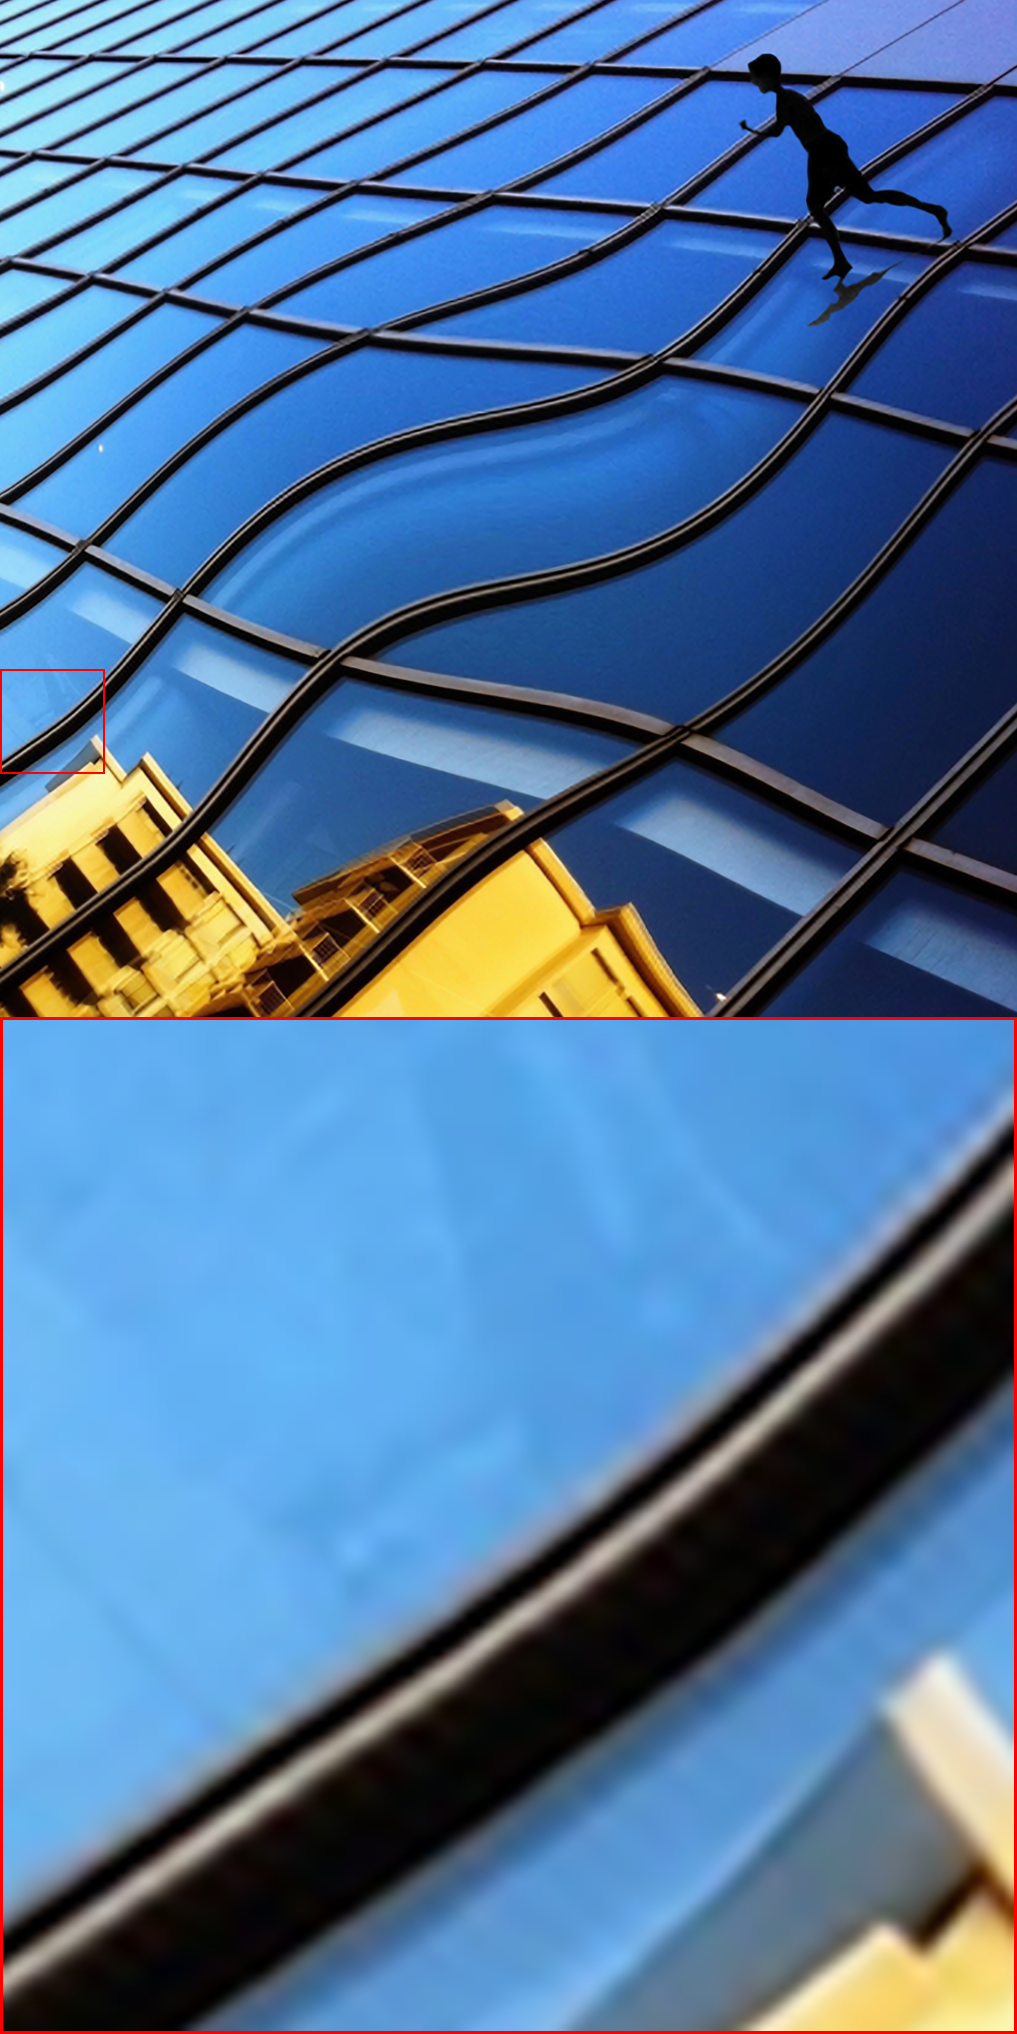
\includegraphics[width=0.15\textwidth]{img082_for_fig2_SelfEx.png}}
& {\graphicspath{{figs/fig2/}}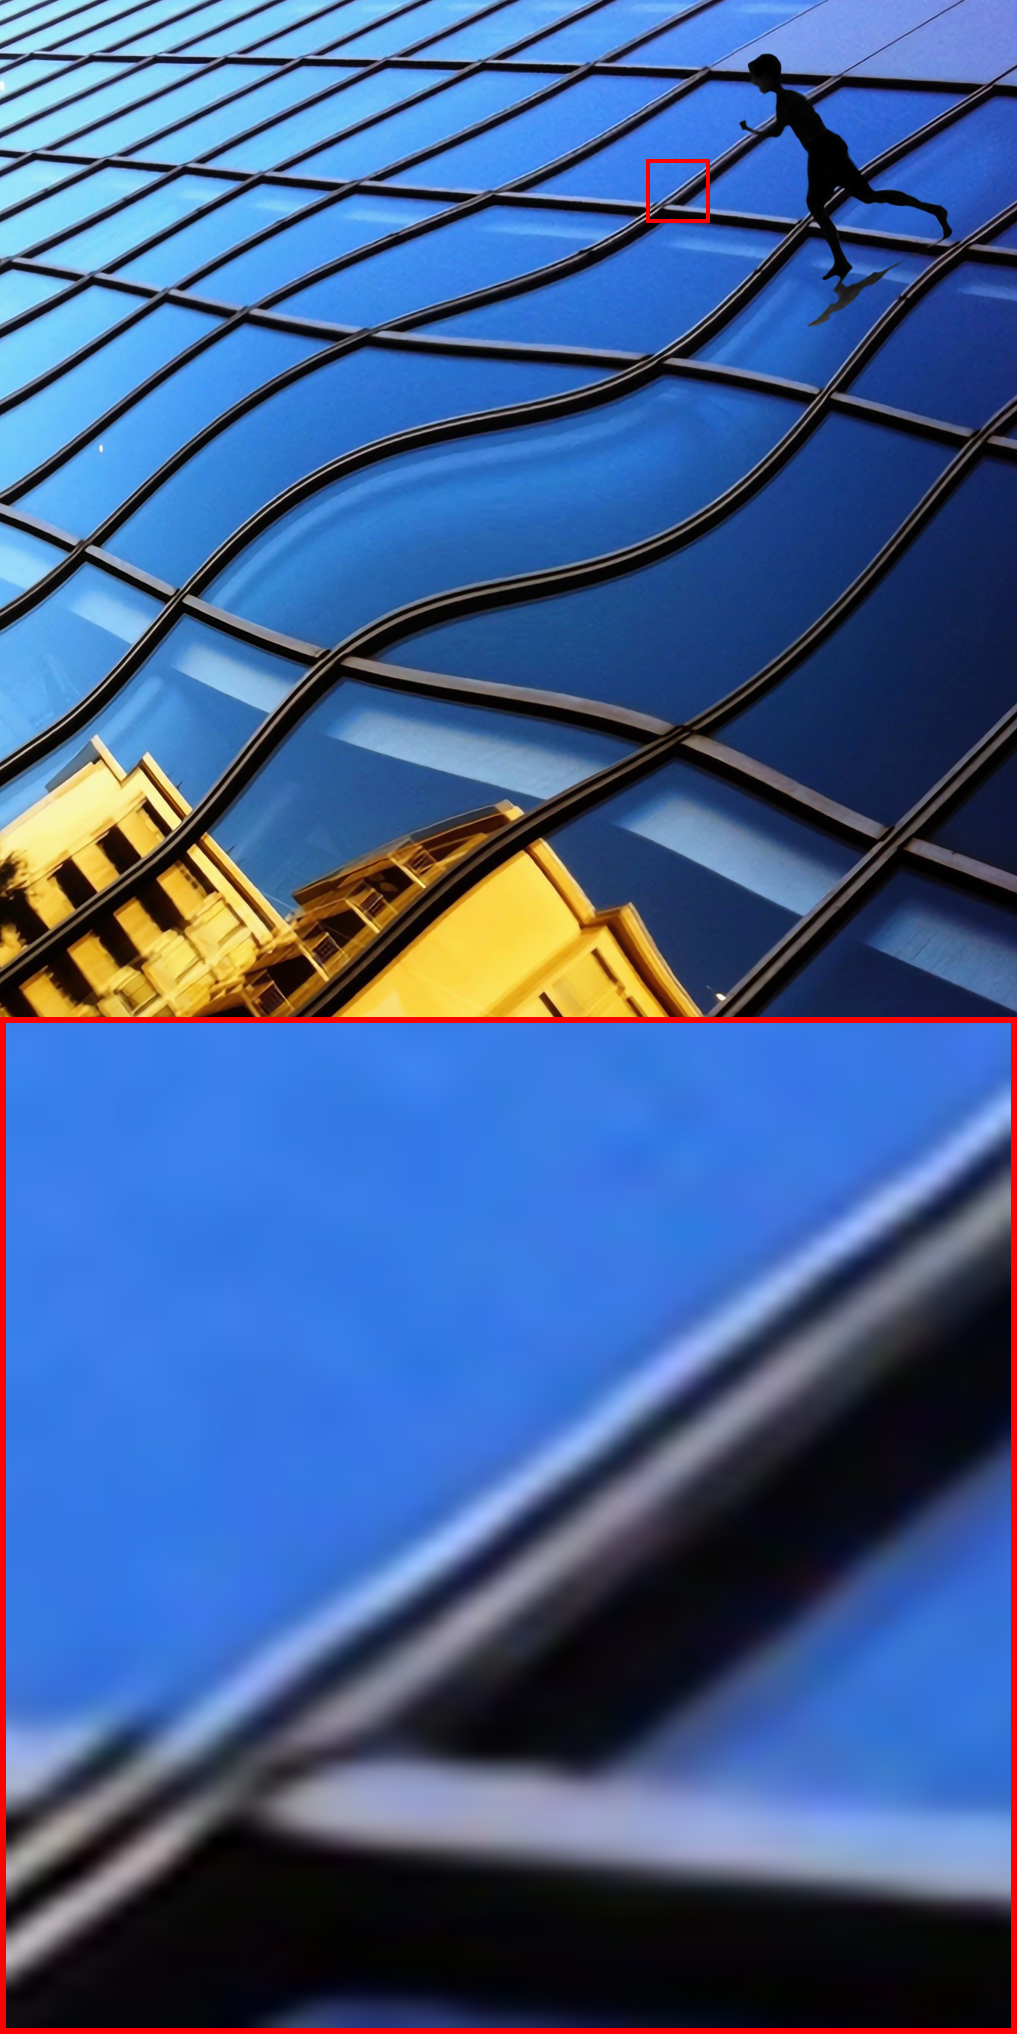
\includegraphics[width=0.15\textwidth]{img082_for_fig2_RCN.png}}
\\
Original& A+& SRCNN& RFL& SelfEx& DRCN (Ours) \\
(PSNR, SSIM)& (32.49, 0.9425)& (32.59, 0.9409)& (32.35, 0.9389)& (33.21, 0.9453)& (34.77, 0.9563)\\
\end{tabular}
\caption{Super-resolution results of ``img082"(Urban100) with scale factor $\times$3. Our result is visually pleasing.}
\label{fig:img2}
\end{center}
\end{adjustwidth}
\end{figure*}

\begin{figure*}
\begin{adjustwidth}{0.5cm}{0.5cm}
\begin{center}
\small
\setlength{\tabcolsep}{3pt}
\begin{tabular}{  c  c  c  c  c  c  }
{\graphicspath{{figs/fig2/}}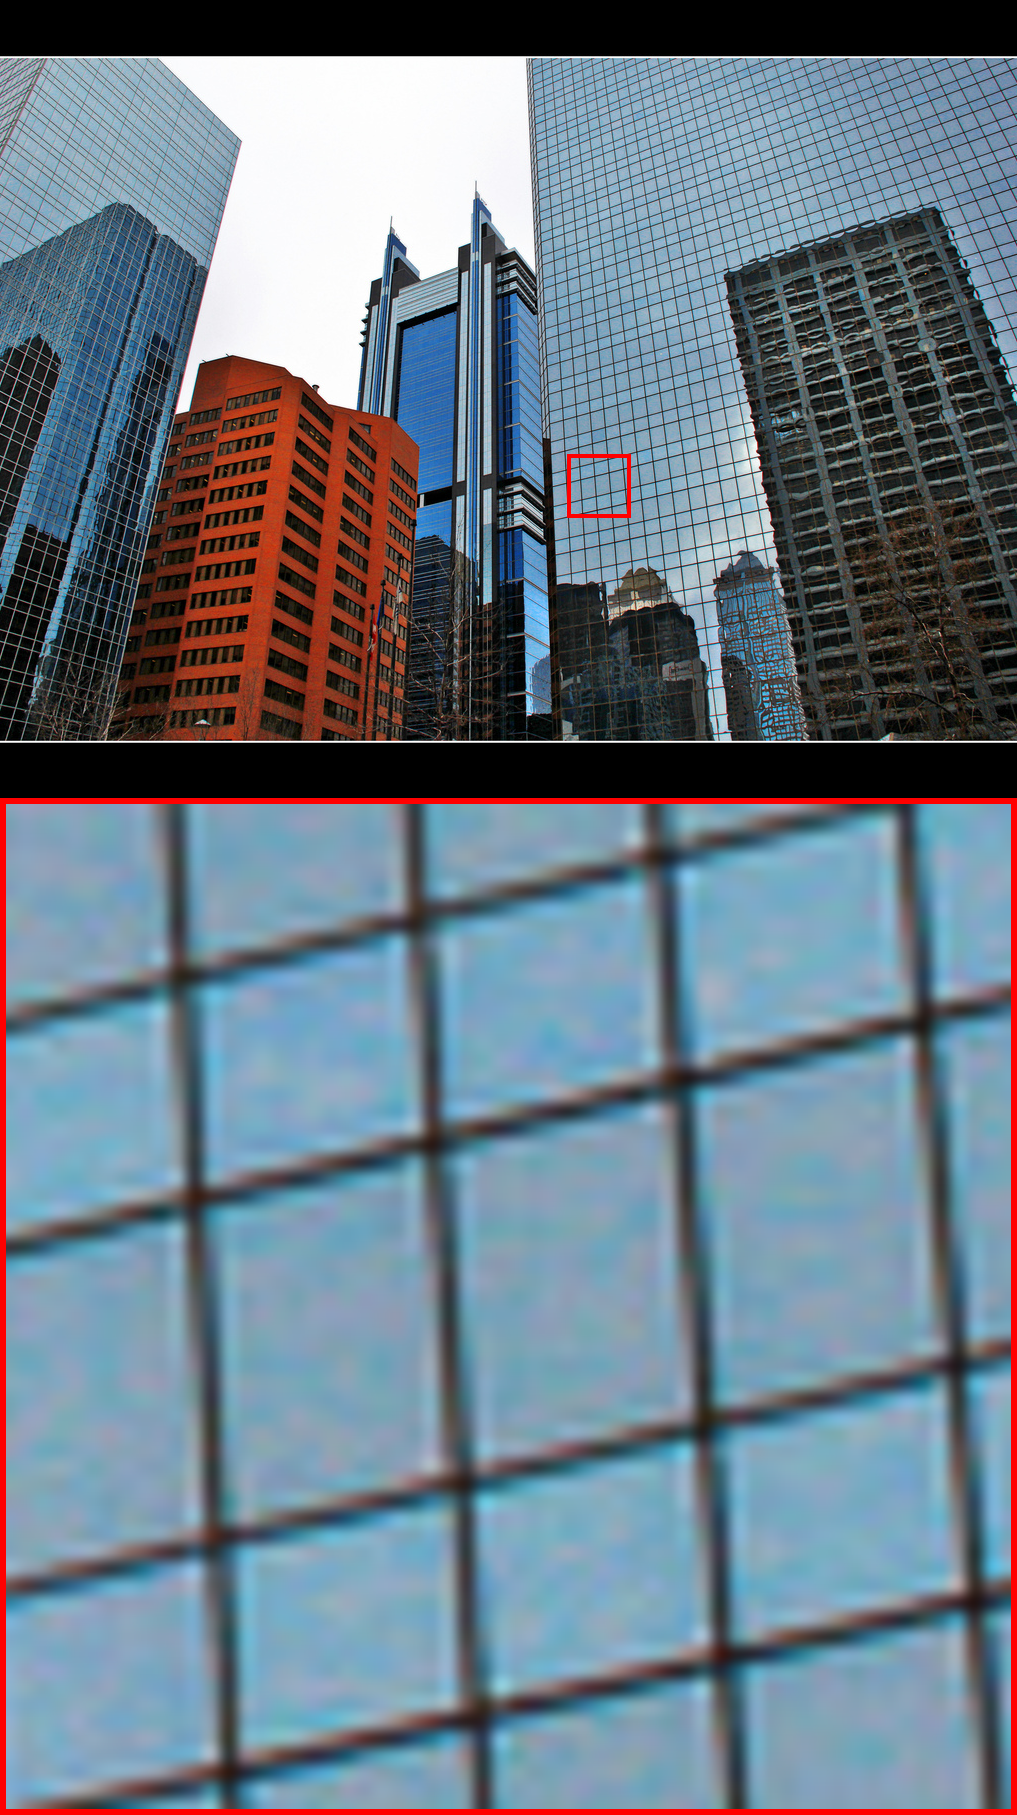
\includegraphics[width=0.15\textwidth]{img099_for_fig2_HR.png}}
& {\graphicspath{{figs/fig2/}}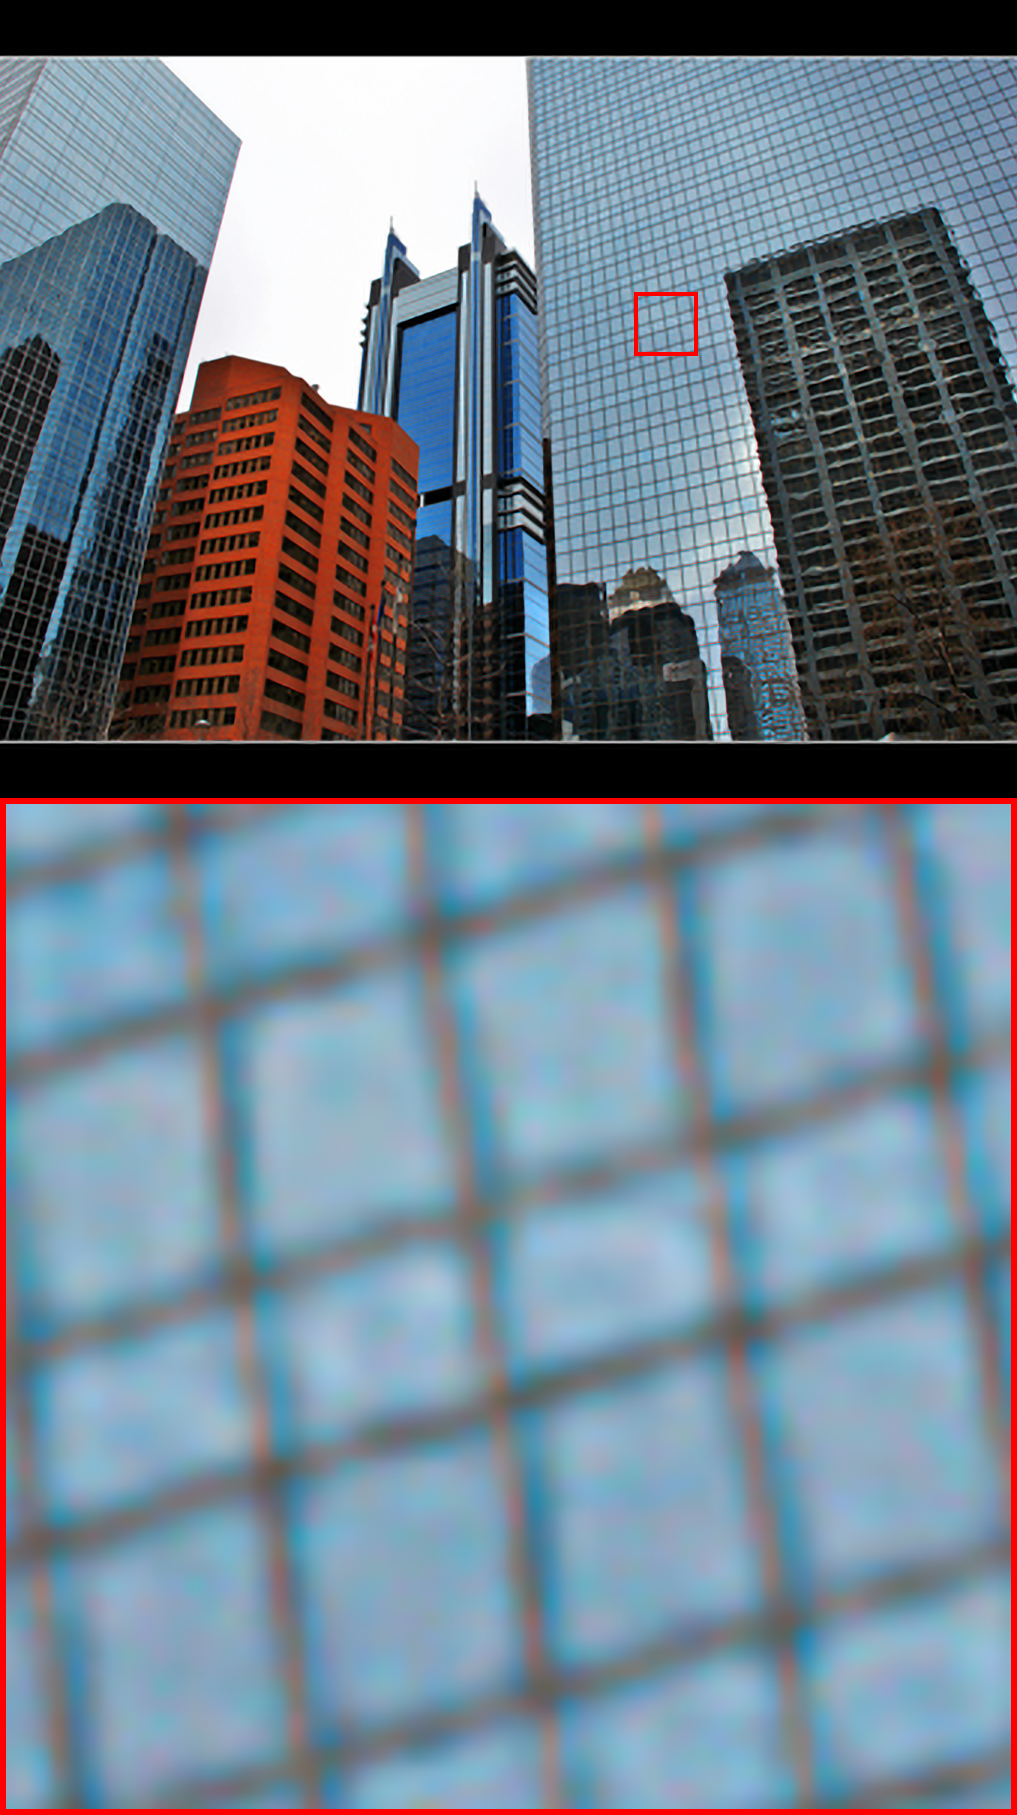
\includegraphics[width=0.15\textwidth]{img099_for_fig2_A+.png}}
& {\graphicspath{{figs/fig2/}}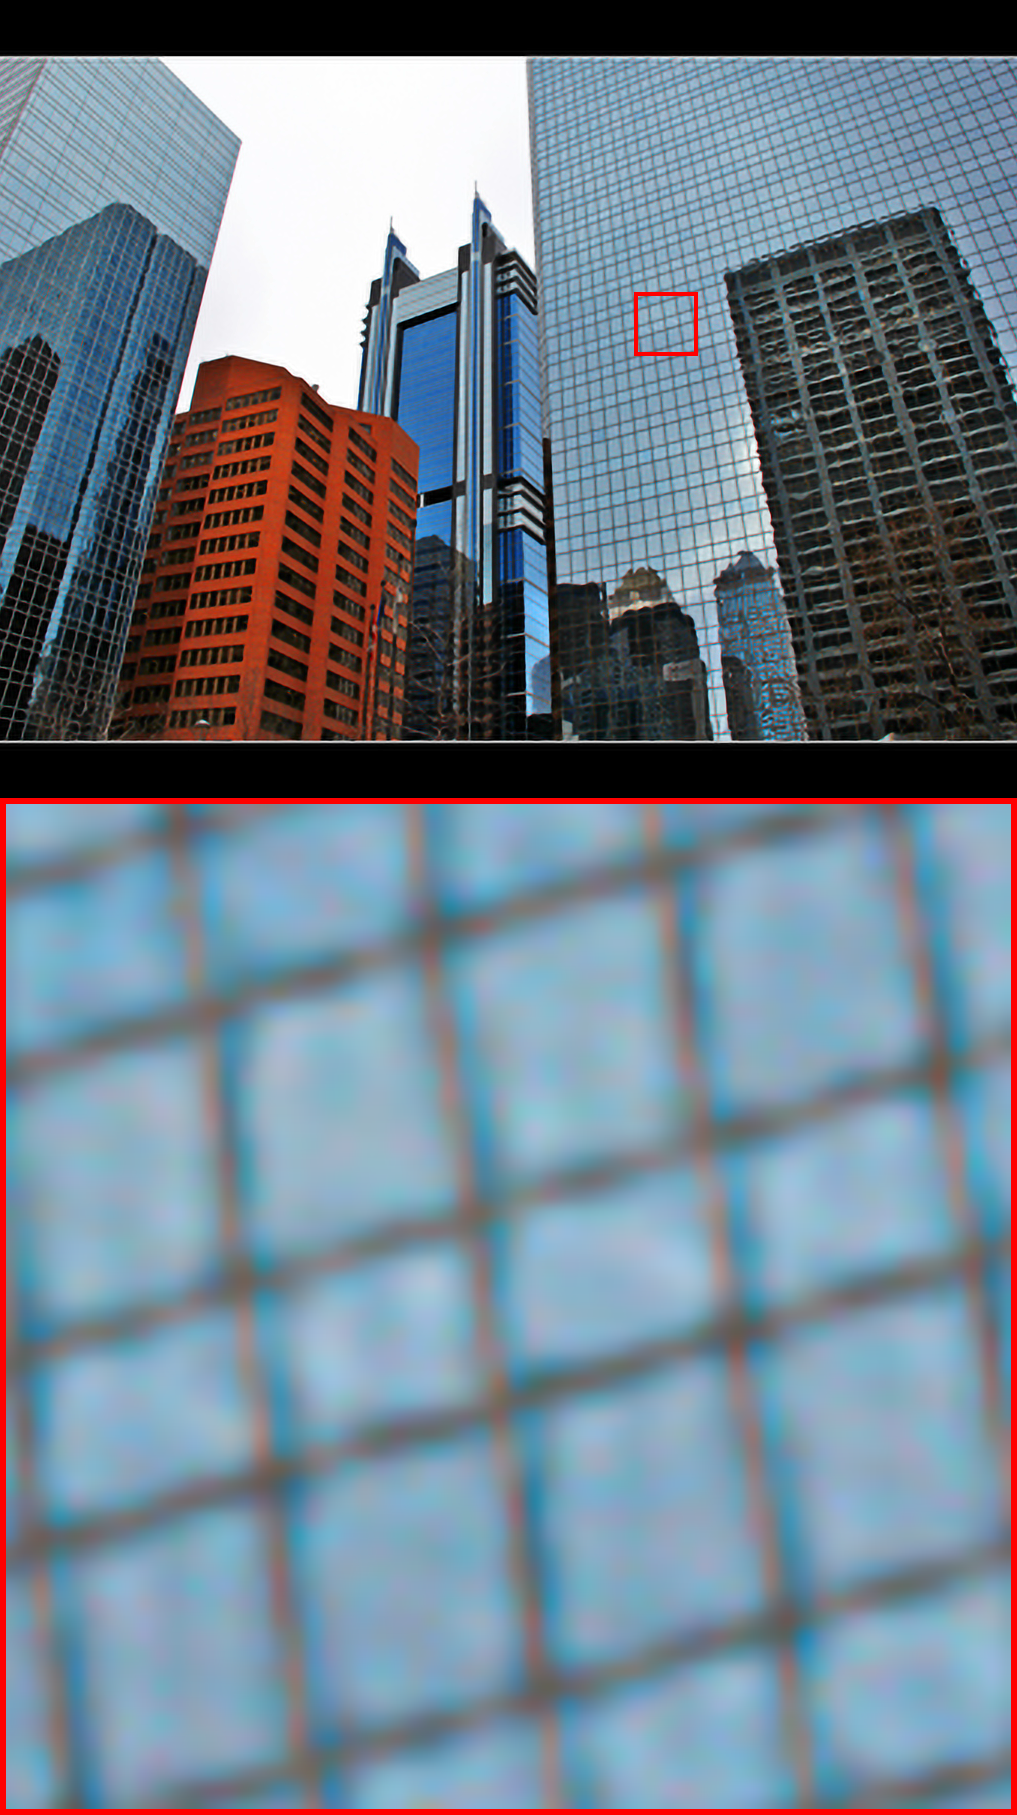
\includegraphics[width=0.15\textwidth]{img099_for_fig2_SRCNN.png}}
& {\graphicspath{{figs/fig2/}}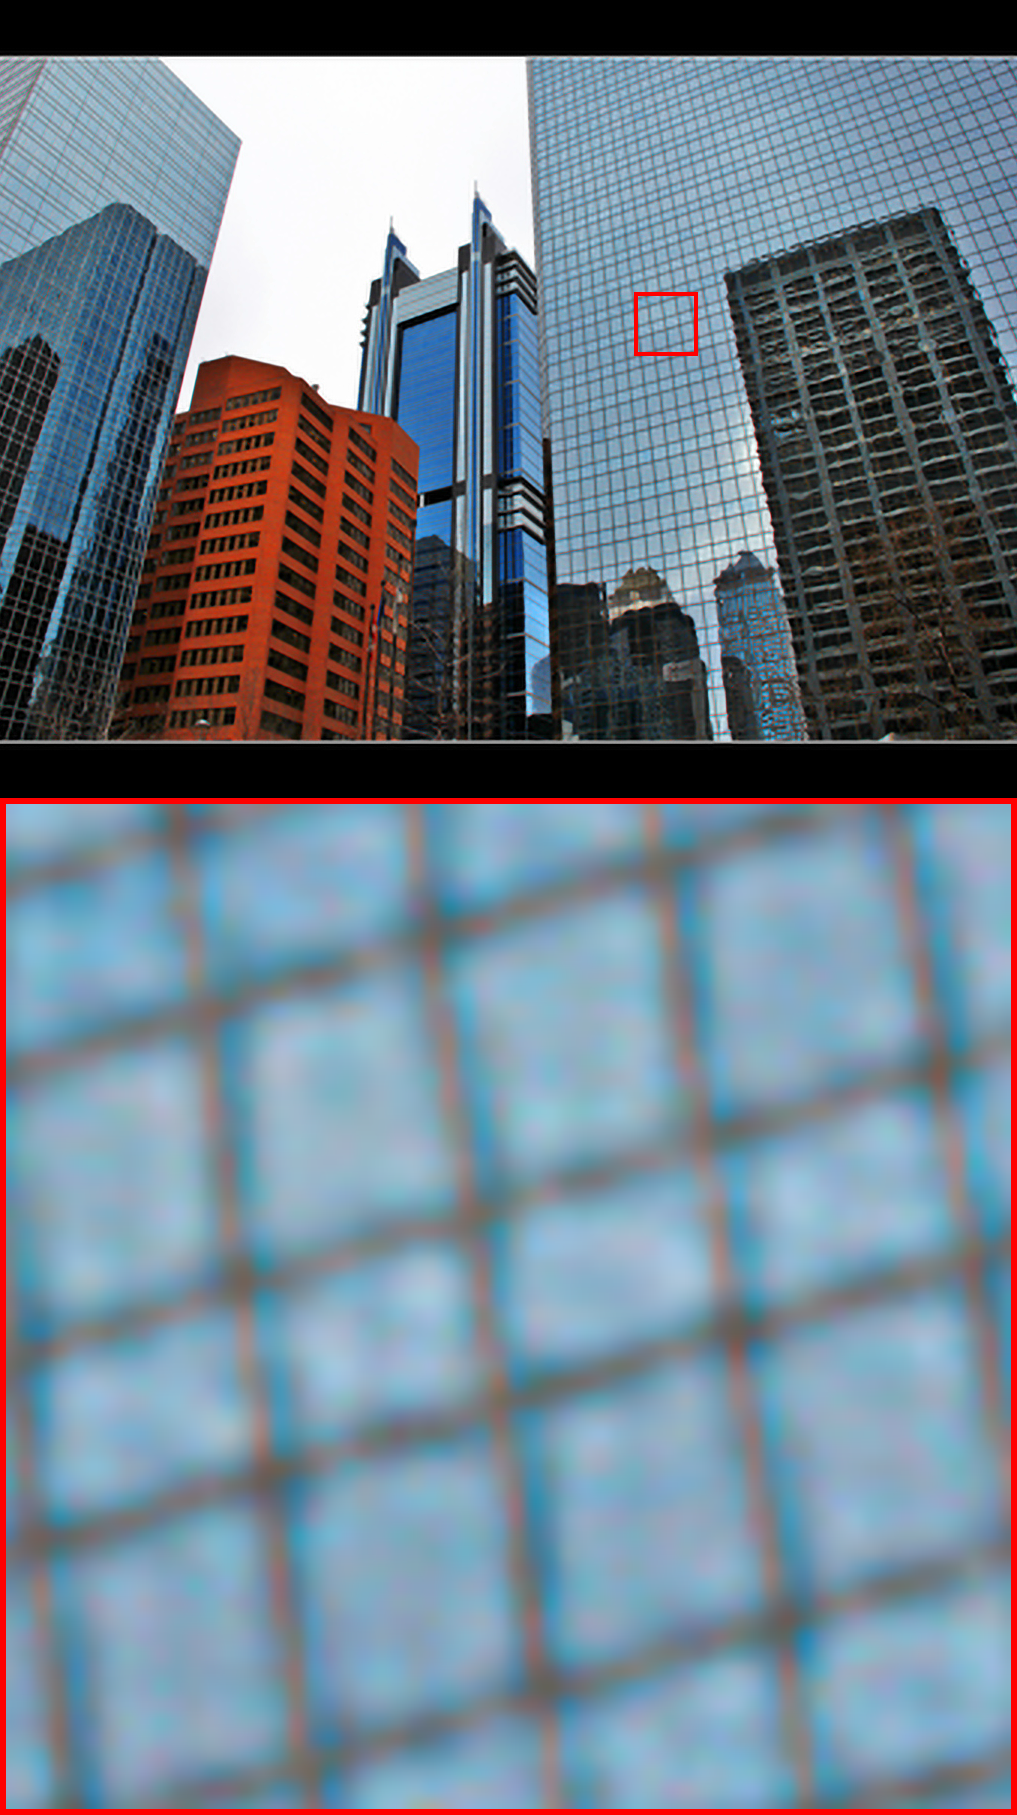
\includegraphics[width=0.15\textwidth]{img099_for_fig2_RFL.png}}
& {\graphicspath{{figs/fig2/}}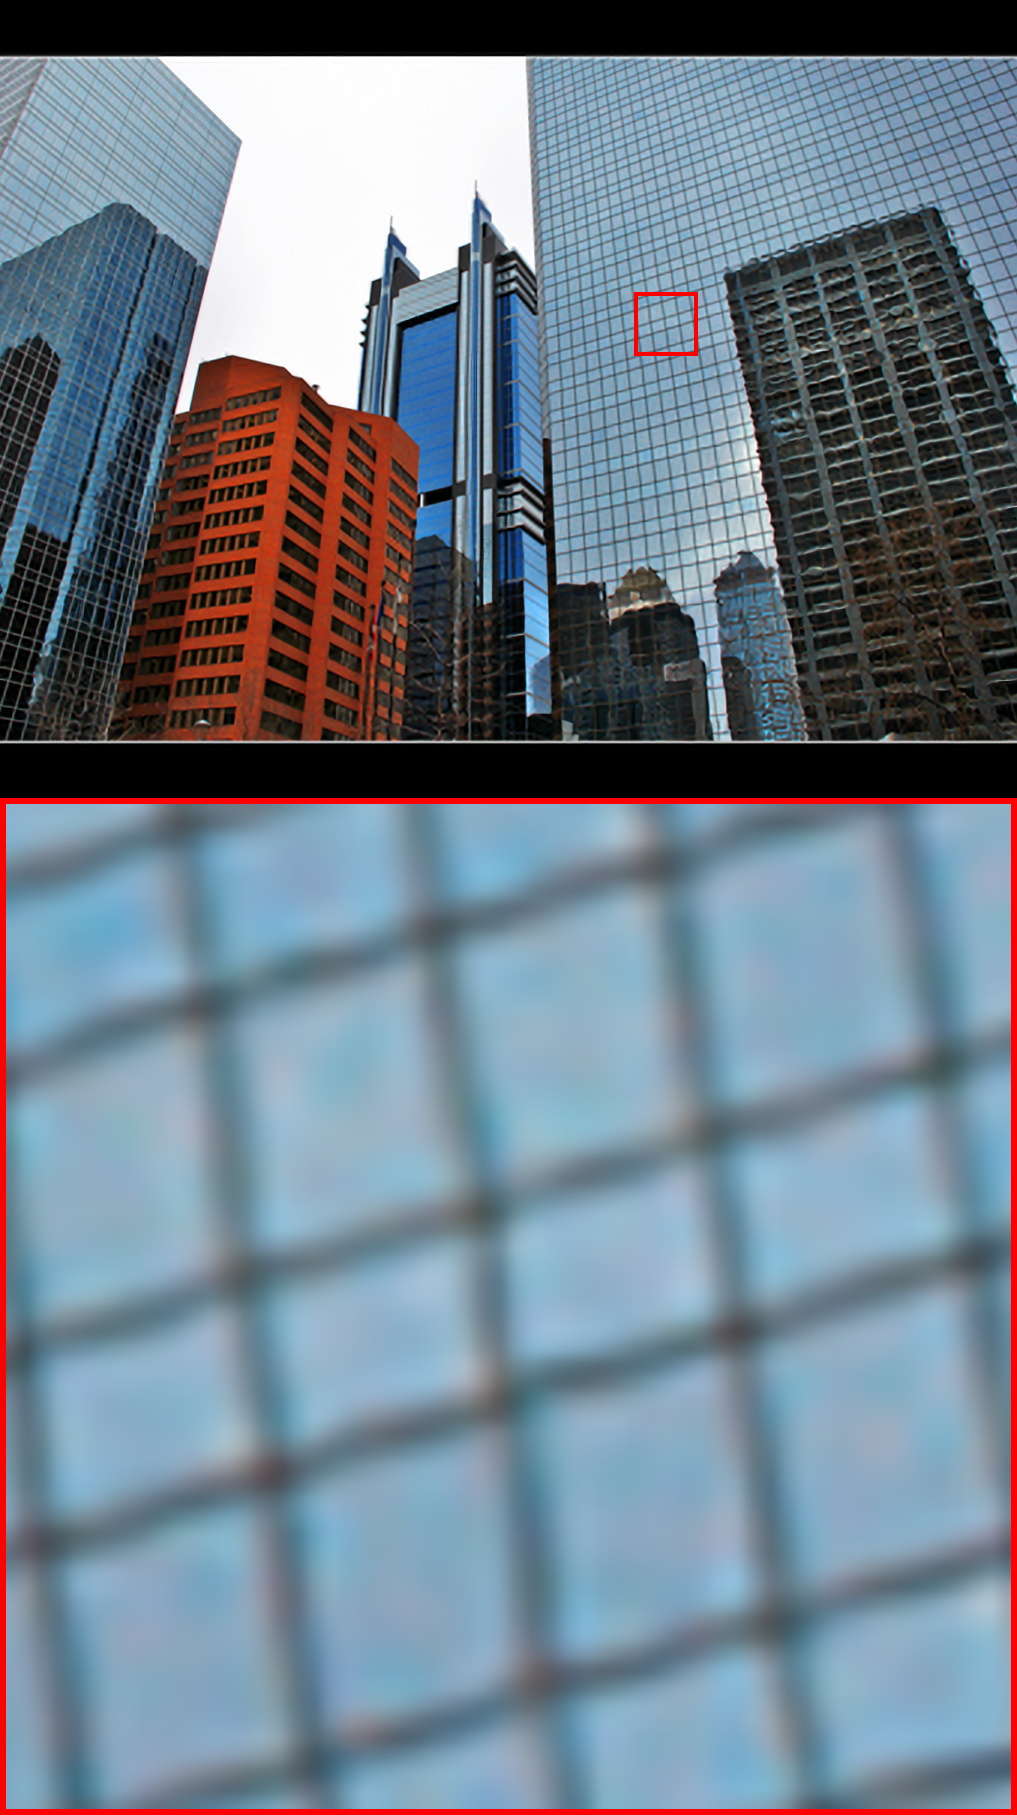
\includegraphics[width=0.15\textwidth]{img099_for_fig2_SelfEx.png}}
& {\graphicspath{{figs/fig2/}}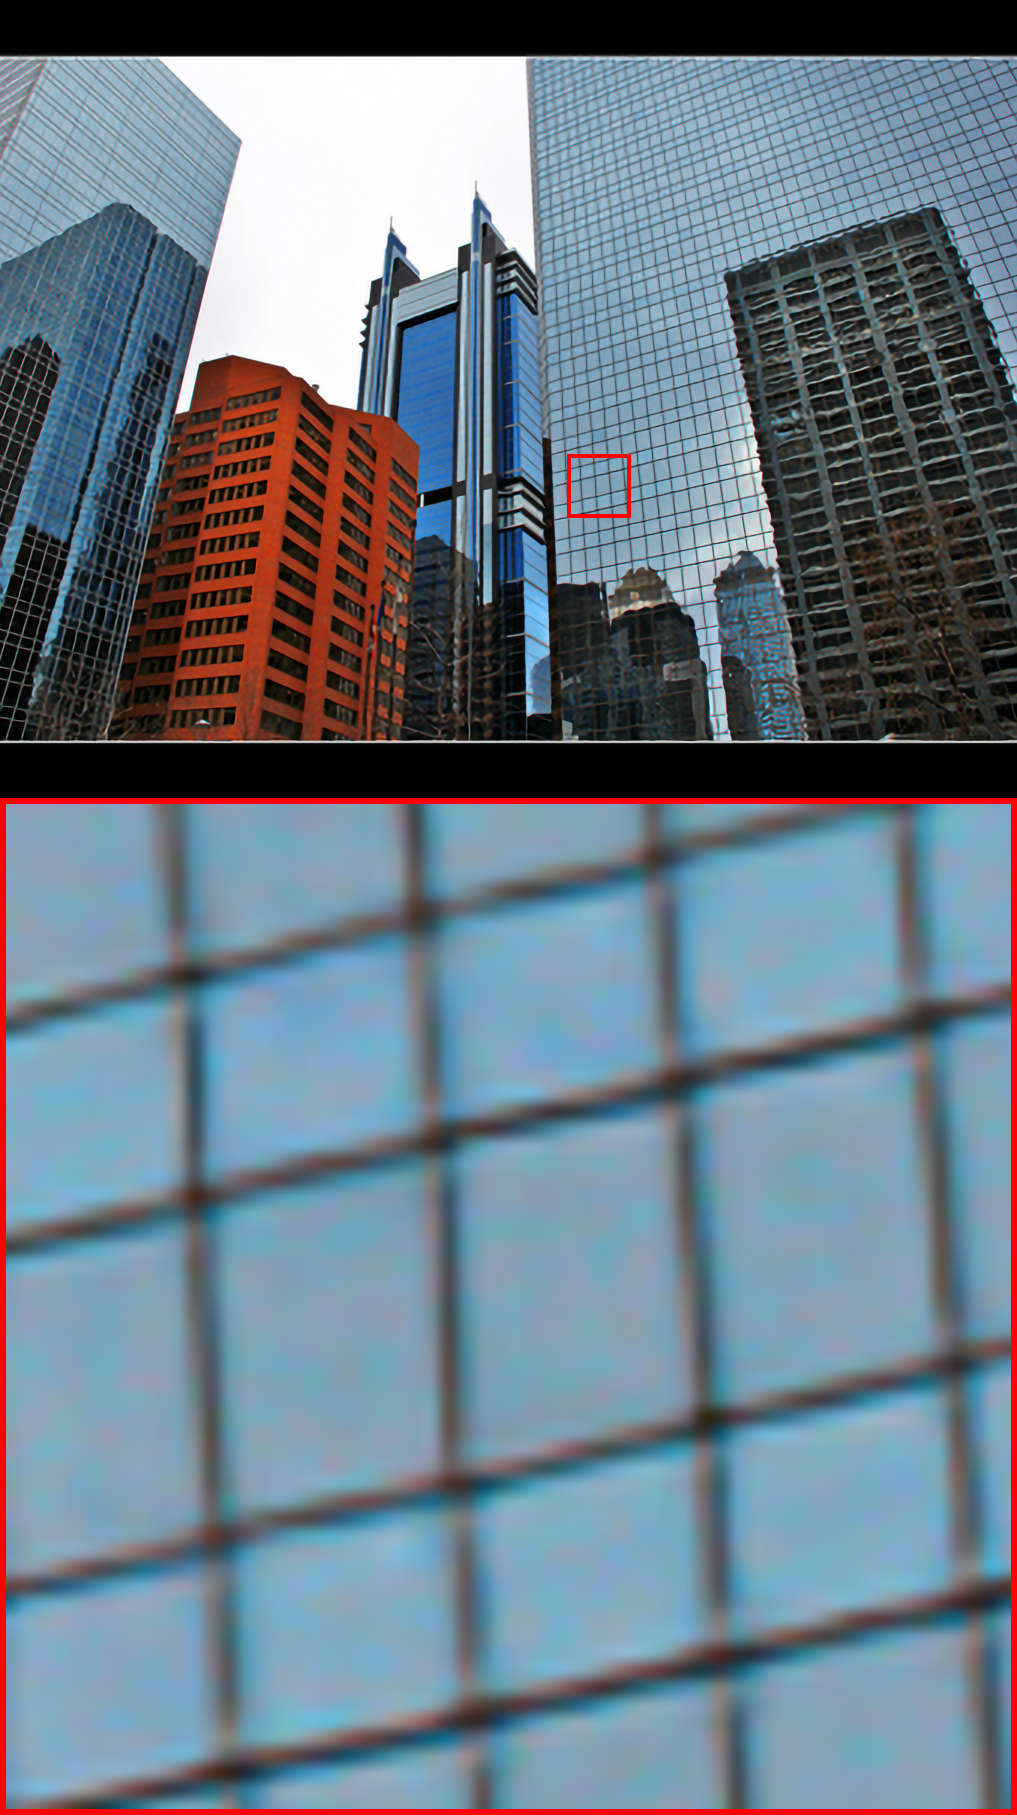
\includegraphics[width=0.15\textwidth]{img099_for_fig2_RCN.png}}
\\
Original& A+& SRCNN& RFL& SelfEx& DRCN (Ours) \\
(PSNR, SSIM)& (24.97, 0.7606)& (25.49, 0.7710)& (24.53, 0.7460)& (25.65, 0.7921)& (26.42, 0.8238)\\
\end{tabular}
\caption{Super-resolution results of ``img099"(Urban100) with scale factor $\times$3. Our result is visually pleasing.}
\label{fig:img3}
\end{center}
\end{adjustwidth}
\end{figure*}

\begin{figure}
\begin{adjustwidth}{0cm}{-0.0cm}
\centering
{\graphicspath{{figs/graph1/}}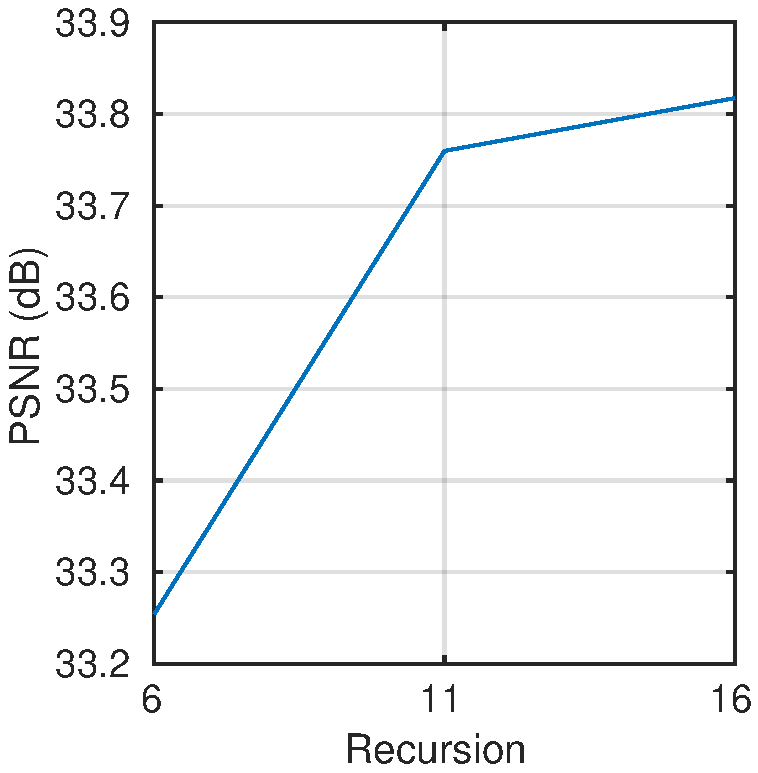
\includegraphics[height=4.8cm]{graphOne.pdf}}
\caption{Recursion versus Performance for the scale factor $\times$3 on the dataset \textit{Set5}. More recursions yielding larger receptive fields lead to better performances. (Graph {\color{red}not complete} yet)}\end{adjustwidth}
\end{figure}
%%%%%%%% Figures End

\subsection{Training}

\textbf{Objective} We now describe the training objective used to find optimal parameters of our model. Given a training dataset $\{{\bf x}^{(i)},{\bf y}^{(i)}\}{}_{i=1}^{N}$, our goal is to find the best model $f$ that accurately predicts values $\mathbf{\hat{y}}=f(\mathbf{x})$.

In the least-squares regression setting, typical in SR, the mean squared error $\frac{1}{2}||\mathbf{y}-f(\mathbf{x})||^{2}$
averaged over the training set is minimized. This favors high Peak Signal-to-Noise
Ratio (PSNR), a widely-used evaluation criteria. 

With recursive-supervision, we have $D+1$ objectives to minimize: supervising $D$ outputs from recursions and the final output. For intermediate outputs, we have the loss function 
\begin{equation}
l_1(\theta) = \sum_{d=1}^D \sum_{i=1}^N \frac{1}{2DN}||{\bf y}^{(i)} -  \hat{\bf y}_d^{(i)} ||^{2},
\end{equation}
where $\theta$ denotes the parameter set and $\hat{\bf y}_d^{(i)}$ is the output from the $d$-th recursion. For the final output, we have 
\begin{equation}
l_2(\theta) = \sum_{i=1}^N \frac{1}{2N}||{\bf y}^{(i)} -  \sum_{d=1}^D  w_d \cdot \hat{\bf y}_d^{(i)} ||^{2}
\end{equation}

Now we give the final loss function $L(\theta)$. The training is regularized by weight decay ($L_2$ penalty multiplied by $\beta$). 
\begin{equation}
L(\theta)  =\alpha  l_1(\theta) + (1 - \alpha) l_2(\theta) + \beta ||\theta||^2,
\end{equation}
where $\alpha$ denotes the importance of the companion objective on the intermediate outputs and $\beta$ denotes the multiplier of weight decay.   Setting $\alpha$ high makes the training procedure stable as early recursions easily converge. As training progresses, $\alpha$ decays to boost the performance of the final output. 

Training is carried out by optimizing the regression objective using mini-batch gradient descent based on back-propagation (LeCun et al. \cite{lecun1998gradient}). We implement our model using the \textit{MatConvNet}\footnote{\url{ http://www.vlfeat.org/matconvnet/}} package \cite{arXiv:1412.4564}. 


\section{Experimental Results}
In this section, we evaluate the performance of our method on several datasets. We first describe datasets used for training and testing our method. Next, our training setup is given. 

We give several experiments for understanding our model properties. The effect of increasing the number of recursions is investigated and TODO add more experiments.  

Finally, we compare our method with several state-of-the-art methods. 

\subsection{Datasets}
For training, we use 91 images proposed in Yang et al. \cite{yang2010image} for all experiments. For testing, we use four datasets. Datasets \textit{Set5} \cite{bevilacqua2012} and \textit{Set14} \cite{zeyde2012single} are often used for benchmark \cite{Timofte,Timofte2013,dong2014image}. Dataset \textit{B100}  consists of natural images in the Berkeley Segmentation Dataset \cite{Martin2001}. Finally, dataset \textit{Urban100}, urban images recently provided by Huang et al. \cite{Huang-CVPR-2015}, is very interesting as it contains many challenging images failed by existing methods.
\subsection{Training Setup}
%
%Training deep models often fail to converge. He et al. \cite{he2015delving} uses a theoretically sound initialization method which helps very deep models converge when training from scratch and they succeed in training 30 weight layers. They, however, report no benefit from training extremely deep models for their problem. In our work, adding layers are beneficial in general. For large scale factors, deep models exploiting contextual information spread in very large field are dominant. 
%
%Training the multi-scale model is straightforward. Training datasets for several specified scales are combined into one big dataset. We demonstrate in the next section that a model learned with this works under multiple scales.  
%
%\textcolor{red}{Data preparation is similar to SRCNN \cite{Dong2014} with some differences. Input patch size is equal to the size of receptive field and images are divided into sub-images with no overlap. 64 sub-images constitue a mini-batch, where sub-images from different scales can be in the same batch.}
%
%
%

We use 16 recursions unless stated otherwise. When unfolded, the longest chain from the input to the output passes 20 conv. layers (receptive field of 41 by 41). We set the momentum parameter to 0.9 and weight decay to 0.0001. Training images are split into 41 by 41 patches with stride 21 and 64 patches are used as a mini-batch for stochastic gradient descent. 

For initializing weights in non-recursive layers, we use the method described in He et al. \cite{he2015delving}. For recursive convolutions, we set all weights to zero except self-connections (connection to the same neuron in the next layer) \cite{socher2012semantic, le2015simple}.  Biases are set to zero.

Learning rate is initially set to 0.01 and then decreased by a factor of 10 if the validation error does not decrease for 5 epochs. If learning rate is less than $10^{-6}$ the procedure is terminated. Training roughly takes 6 days on a machine using one Titan X GPU. 


\subsection{Comparisons with State-of-the-Art Methods}
We provide quantitative and qualitative comparisons. For benchmark, we use public code for A+ \cite{Timofte}, SRCNN \cite{dong2014image}, RFL \cite{schulter2015fast} and  Huang et al. \cite{Huang-CVPR-2015}. We deal with luminance components only as similarly done in other methods because human is much more sensitive to see details in intensity than in color. 

As  some methods such as A+ \cite{Timofte} and  RFL \cite{schulter2015fast} do not predict image boundary, they require cropping pixels near borders. For our method, this procedure is unnecessary as our network predicts the full-sized image. For fair comparison, however, we also crop pixels to the same amount. PSNRs can be slightly different from original papers as existing methods use slightly different evaluation frameworks. We use the public evaluation code used in \cite{Huang-CVPR-2015}.

In Table \ref{tbl:benchmark}, we provide a summary of quantitative evaluation on several datasets. 
Our method outperforms all existing methods in all datasets and scale factors (both PSNR and SSIM). In Figures \ref{fig:img1}, \ref{fig:img2} and \ref{fig:img3}, example images are given. Our method produces relatively sharp edges respecting patterns. In contrast, edges in other images are blurred.

\section{Conclusion}
In this work, we have presented a super-resolution method using a deeply-recursive convolutional network. Our network efficiently reuses weight parameters while exploiting a large image context. To ease the difficulty of training the model, we use recursive-supervision and skip-connection. We have demonstrated that our method outperforms existing methods by a large margin on benchmarked images. In the future, one can try more recursions in order to use image-level context. We believe our approach is readily applicable to other image restoration problems such as denoising and compression artifact removal.

%\clearpage
{\small
	\bibliographystyle{ieee}
	\bibliography{DRCN}
}
\end{document}